%% For double-blind review submission, w/o CCS and ACM Reference (max submission space)
%\documentclass[acmsmall,review,anonymous]{acmart}\settopmatter{printfolios=true,printccs=false,printacmref=false}
%% For double-blind review submission, w/ CCS and ACM Reference
%\documentclass[acmsmall,review,anonymous]{acmart}\settopmatter{printfolios=true}
%% For single-blind review submission, w/o CCS and ACM Reference (max submission space)
%\documentclass[acmsmall,review]{acmart}\settopmatter{printfolios=true,printccs=false,printacmref=false}
%% For single-blind review submission, w/ CCS and ACM Reference
%%\documentclass[acmsmall,review]{acmart}\settopmatter{printfolios=true}
%% For final camera-ready submission, w/ required CCS and ACM Reference
%%\documentclass[acmsmall]{acmart}\settopmatter{}
%% Actual final camera-ready submission command from Conference-Publishing.com
\documentclass[acmsmall,screen]{acmart} 

%%%
%%% The following is specific to HOPL '20 and the paper
%%% 'The Origins of Objective-C at PPI/Stepstone and Its Evolution at NeXT'
%%% by Brad Cox, Steve Naroff, and Hansen Hsu.
%%%
\setcopyright{rightsretained} 
\acmJournal{PACMPL}
\acmYear{2020} \acmVolume{4} \acmNumber{HOPL} \acmArticle{82} \acmMonth{6} \acmPrice{}\acmDOI{10.1145/3386332}
\copyrightyear{2020}

%% Used to acknowledge ACM HOPL Paper shepherd
\usepackage{acmshepherd}
%% For Non-archival references to conform with new HOPL style guidelines
\usepackage{acmNArefs}
%% For better typesetting quality
\usepackage{microtype}


%% Bibliography style
\bibliographystyle{ACM-HOPL-Reference-Format}
\bibliographystyleNA{ACM-HOPL-Reference-Format}
\citestyle{acmauthoryear}   %% For author/year citations


%%%%%%%%%%%%%%%%%%%%%%%%%%%%%%%%%%%%%%%%%%%%%%%%%%%%%%%%%%%%%%%%%%%%%%
%% Note: Authors migrating a paper from PACMPL format to traditional
%% SIGPLAN proceedings format must update the '\documentclass' and
%% topmatter commands above; see 'acmart-sigplanproc-template.tex'.
%%%%%%%%%%%%%%%%%%%%%%%%%%%%%%%%%%%%%%%%%%%%%%%%%%%%%%%%%%%%%%%%%%%%%%


%% Some recommended packages.
\usepackage{booktabs}   %% For formal tables:
                        %% http://ctan.org/pkg/booktabs
\usepackage{subcaption} %% For complex figures with subfigures/subcaptions
                        %% http://ctan.org/pkg/subcaption

%% added for non-breaking dashes
\usepackage[shortcuts]{extdash}
%% needed for multipage table
\usepackage{longtable}
%% needed to insert SNaroff PDF document in appendix
\usepackage{pdfpages}
%% used to add offsets to page numbers returned by pageref
\usepackage{refcount}

%% to get rid of orphans and widows
\clubpenalty = 10000
\widowpenalty = 10000
\displaywidowpenalty = 10000

\begin{document}

%% Title information
\title[The Origins of Objective-C]{The Origins of Objective-C at PPI/Stepstone and Its Evolution at NeXT}         %% [Short Title] is optional;
                                        %% when present, will be used in
                                        %% header instead of Full Title.
%\titlenote{with title note}             %% \titlenote is optional;
                                        %% can be repeated if necessary;
                                        %% contents suppressed with 'anonymous'
%\subtitle{Subtitle}                     %% \subtitle is optional
%\subtitlenote{with subtitle note}       %% \subtitlenote is optional;
                                        %% can be repeated if necessary;
                                        %% contents suppressed with 'anonymous'


%% Author information
%% Contents and number of authors suppressed with 'anonymous'.
%% Each author should be introduced by \author, followed by
%% \authornote (optional), \orcid (optional), \affiliation, and
%% \email.
%% An author may have multiple affiliations and/or emails; repeat the
%% appropriate command.
%% Many elements are not rendered, but should be provided for metadata
%% extraction tools.

%% Author with single affiliation.
\author{Brad J. Cox}
%\authornote{with author1 note}          %% \authornote is optional;
                                        %% can be repeated if necessary
%\orcid{nnnn-nnnn-nnnn-nnnn}             %% \orcid is optional
\affiliation{
%  \position{Position1}
%  \department{Department1}              %% \department is recommended
  \institution{Retired}            %% \institution is required
%  \streetaddress{994 Bent Tree Lane}
%  \city{Manassas}
%  \state{VA}
%  \postcode{20111}
  \country{USA}                    %% \country is recommended
}
\email{bradjcox@gmail.com}          %% \email is recommended

%% Second Author with affiliations and emails.
\author{Steve Naroff}
%\authornote{with author2 note}          %% \authornote is optional;
                                        %% can be repeated if necessary
%\orcid{nnnn-nnnn-nnnn-nnnn}             %% \orcid is optional
\affiliation{
%  \position{Position2a}
%  \department{Department2a}             %% \department is recommended
  \institution{Retired}           %% \institution is required
%  \streetaddress{367 West Del Mar Blvd., Unit \#105}
%  \city{Pasadena}
%  \state{CA}
%  \postcode{91105}
  \country{USA}                   %% \country is recommended
}
\email{naroff@me.com}         %% \email is recommended

% Third author
\author{Hansen Hsu}
%\authornote{with author2 note}          %% \authornote is optional;
                                        %% can be repeated if necessary
\orcid{0000-0002-5572-5987}             %% \orcid is optional
\affiliation{
  \position{Curator}
  \department{Software History Center}             %% \department is recommended
  \institution{Computer History Museum}           %% \institution is required
  \streetaddress{1401 N. Shoreline Blvd.}
  \city{Mountain View}
  \state{CA}
  \postcode{94043}
  \country{USA}                   %% \country is recommended
}
\email{hhsu@computerhistory.org}         %% \email is recommended

\shepherd{Shigeru Chiba, University of Tokyo, Japan}

%% Abstract
%% Note: \begin{abstract}...\end{abstract} environment must come
%% before \maketitle command
\begin{abstract}
%The prehistory of Objective-C starts at ITT in the early 1980s as OOPC (Object-oriented Pre-Compiler), in a group that included Tom Love and Brad Cox, who were investigating the use of object-oriented techniques to improve productivity by 10x in organizations. Love and Cox were intrigued by Smalltalk's features but wanted it to be compatible with the Unix and C environments used by IT&T. Cox quickly wrote up a pre-compiler that would translate a Smalltalk-like syntax into C. Love felt there was a market for object-oriented solutions that could coexist with legacy languages and platforms, and after a brief stint at Schlumberger-Doll, co-founded with Cox, Productivity Products International (PPI), later Stepstone, to pursue this. Cox developed the ideas behind OOPC into a full compiled language: Objective-C. Cox saw Objective-C as a crucial link in his larger vision of creating a market for ``pre-fabricated'' software components, which could be bought off the shelf and would make software development more like hardware development. ``Fabrication'' of components would be done in C, with Objective-C serving as the ``soldering gun'' to knit these ``software ICs'' together. Thus Objective-C was originally a minimalist design. Modeled after Smalltalk, the focus was a modest language to support the development of C-based components. By contrast, C++ was ambitious and considered to be the next iteration of the C programming language.  While both Objective-C and C++ embrace C, they do so in very different ways. Stepstone's business model was to sell the software components, not the language itself. As such, after acquiring venture funding and hiring a programming staff, which included Steve Naroff, Cox shifted to focus on the component products, “ICpaks.'' 
%Steve Naroff joined Stepstone in 1986 with experience in both C and MAILSAIL. In 1987, with Alan Watt, Naroff drafted a plan for further work on Objective-C, with Naroff focusing on improving C integration, while Watt focused on new features from Smalltalk, such as blocks. In 1987, both NeXT and HP became adopters of Objective-C, but for different reasons. HP wanted it for research and prototyping, and pushed for features such as garbage collection, while NeXT was focused on pragmatic development and deployment issues, and moreover, wanted a language that it could mold to conform to its needs. Naroff became the primary engineer addressing NeXT's needs in the language at Stepstone. Naroff solved a fragility issue with selectors and added explicit declaration constructs. Naroff interfaced with NeXT engineers and, impressed with their work, decided to leave Stepstone for NeXT in 1988. Once at NeXT, Naroff added Objective-C to Richard Stallman's GNU GCC compiler, removing the need for a preprocessor, making NeXT one of the first commercial companies to use GCC. In 1989, Naroff added an extension mechanism to Objective-C, known as ``categories.'' In 1989-90, Naroff added the ability to mix Objective-C and C++ code, the combination of which became known as ``Objective-C++.'' Also in 1990, Naroff modified GCC to emit method signatures, Bertrand Serlet began developing method forwarding, and Serlet and Blaine Garst developed protocols (now known as ``interfaces'' in Java) to provide multiple inheritance of interface but not implementation.
The roots of Objective-C began at ITT in the early 1980s in a research group led by Tom Love investigating improving programmer productivity by an order of magnitude, a concern motivated by the perceived ``software crisis'' articulated in the late 1960s. In 1981, Brad Cox, a member of this group, began to investigate Smalltalk and object-oriented programming for this purpose, but needed a language compatible with the Unix and C environments used by ITT. That year, Cox quickly wrote up the Object-Oriented Pre-Compiler (OOPC) that would translate a Smalltalk-like syntax into C.

Love felt there was a market for object-oriented solutions that could coexist with legacy languages and platforms, and after a brief stint at Schlumberger-Doll, co-founded with Cox Productivity Products International (PPI), later renamed as Stepstone, to pursue this. At PPI, Cox developed OOPC into Objective-C. Cox saw Objective-C as a crucial link in his larger vision of creating a market for ``pre-fabricated'' software components (``software-ICs''), which could be bought off the shelf and which, Cox believed, would unleash a ``software industrial revolution.'' 

Steve Naroff joined Stepstone in 1986 as Steve Jobs' NeXT Computer became an important customer for Objective-C, as it was being used in its NeXTSTEP operating system. Naroff became the primary Stepstone developer addressing NeXT's issues with Objective-C, solving a key fragility problem preventing NeXT from deploying forwards-compatible object libraries. Impressed with NeXT, Naroff left Stepstone for NeXT in 1988, and once there, added Objective-C support to Richard Stallman's GNU GCC compiler, which NeXT was using as its C compiler, removing the need to use Stepstone's ObjC to C translator. Over the next several years, Naroff and others would add significant new features to Objective-C, such as ``categories,'' ``protocols,'' and the ability to mix in C++ code. When Stepstone folded in 1994, all rights to Objective-C were acquired by NeXT. This eventually transferred to Apple when NeXT was acquired by Apple in 1997. Objective-C became the basis for Apple's Mac OS X and then iOS platforms, and Naroff and others at Apple added additional features to the language in the late 2000s as the iPhone App Store greatly expanded Objective-C's user base.
\end{abstract}


%% 2012 ACM Computing Classification System (CSS) concepts
%% Generate at 'http://dl.acm.org/ccs/ccs.cfm'.
\begin{CCSXML}
<ccs2012>
    <concept>
        <concept_id>10011007.10011006.10011008</concept_id>
        <concept_desc>Software and its engineering~General programming languages</concept_desc>
        <concept_significance>500</concept_significance>
        </concept>
<concept>
   <concept>
       <concept_id>10011007.10011006.10011008.10011009.10011011</concept_id>
       <concept_desc>Software and its engineering~Object oriented languages</concept_desc>
       <concept_significance>500</concept_significance>
       </concept>
   <concept>
       <concept_id>10011007.10011006.10011008.10011024.10011029</concept_id>
       <concept_desc>Software and its engineering~Classes and objects</concept_desc>
       <concept_significance>300</concept_significance>
       </concept>
   <concept>
       <concept_id>10011007.10011006.10011008.10011024.10011026</concept_id>
       <concept_desc>Software and its engineering~Inheritance</concept_desc>
       <concept_significance>300</concept_significance>
       </concept>
   <concept>
       <concept_id>10011007.10011006.10011008.10011024.10011025</concept_id>
       <concept_desc>Software and its engineering~Polymorphism</concept_desc>
       <concept_significance>300</concept_significance>
       </concept>
   <concept>
       <concept_id>10011007.10011006.10011008.10011024.10003202</concept_id>
       <concept_desc>Software and its engineering~Abstract data types</concept_desc>
       <concept_significance>300</concept_significance>
       </concept>
   <concept>
       <concept_id>10011007.10011006.10011041</concept_id>
       <concept_desc>Software and its engineering~Compilers</concept_desc>
       <concept_significance>300</concept_significance>
       </concept>
   <concept>
       <concept_id>10011007.10011006.10011041.10011048</concept_id>
       <concept_desc>Software and its engineering~Runtime environments</concept_desc>
       <concept_significance>300</concept_significance>
       </concept>
   <concept>
       <concept_id>10011007.10011006.10011066.10011067</concept_id>
       <concept_desc>Software and its engineering~Object oriented frameworks</concept_desc>
       <concept_significance>300</concept_significance>
       </concept>
   <concept>
       <concept_id>10003456.10003457.10003521.10003525</concept_id>
       <concept_desc>Social and professional topics~History of programming languages</concept_desc>
       <concept_significance>500</concept_significance>
       </concept>
   <concept>
       <concept_id>10003456.10003457.10003521.10003524</concept_id>
       <concept_desc>Social and professional topics~History of software</concept_desc>
       <concept_significance>100</concept_significance>
       </concept>
 </ccs2012>
\end{CCSXML}

\ccsdesc[500]{Software and its engineering~General programming languages}
\ccsdesc[500]{Software and its engineering~Object oriented languages}
\ccsdesc[300]{Software and its engineering~Classes and objects}
\ccsdesc[300]{Software and its engineering~Inheritance}
\ccsdesc[300]{Software and its engineering~Polymorphism}
\ccsdesc[300]{Software and its engineering~Abstract data types}
\ccsdesc[300]{Software and its engineering~Compilers}
\ccsdesc[300]{Software and its engineering~Runtime environments}
\ccsdesc[300]{Software and its engineering~Object oriented frameworks}
\ccsdesc[500]{Social and professional topics~History of programming languages}
\ccsdesc[100]{Social and professional topics~History of software}
%% End of generated code

%% Keywords
%% comma separated list
\keywords{Objective-C, OOPC, PPI, Stepstone, ITT, NeXT, Apple, message passing, dynamic binding, Smalltalk, C++, software-ICs, software crisis, categories, protocols}  %% \keywords are mandatory in final camera-ready submission


%% \maketitle
%% Note: \maketitle command must come after title commands, author
%% commands, abstract environment, Computing Classification System
%% environment and commands, and keywords command.
\maketitle


\section{Introduction}
\label{sec-Intro}

In 2020, most software developers know of Objective-C as the language used to write software for Apple's iPhone and Macintosh computing platforms. What they may not know is that Objective-C predates the iPhone by two decades, and was not originated by Apple. Objective-C was chosen as the main programming language for NeXTSTEP, the operating system of the NeXT Computer, produced by Steve Jobs' startup NeXT after he left Apple in 1985. It was Apple's purchase of NeXT in 1997, and its development of NeXTSTEP into Mac OS X and later iOS, that made Objective-C central to Apple's technology stack. Yet Objective-C predates even NeXT. Objective-C was created by Brad Cox and Tom Love, the co-founders of a small Connecticut company, Productivity Products International, later renamed Stepstone, to spur the computing industry to adopt object-oriented programming and create a market for software components, which they believed could revolutionize software production by improving programmer productivity by an order of magnitude.

\section{The Context of the ``Software Crisis''}
\label{sec-SoftwareCrisis}
Objective-C had its origins in a technology research group concerned with improving the productivity of software programmers, immersed in the discourse of the ``software crisis.'' Beginning in the 1960s, a growing body of computing literature began to articulate a sense of immanent crisis in the production of software. This literature has been studied by a number of historians of computing, with some arguing that the perceived ``crisis'' was primarily a rhetorical construction \citetext{\citealp {abbate_software_2012, ensmenger_computer_2010, ensmenger_software_2002, mackenzie_mechanizing_2001, mahoney_finding_2004, akera_software:_2002, mahoney_roots_1990, slayton_arguments_2013, tomayko_software_2002}, \citealpNA{haigh_dijkstras_2010}}. Regardless of its reality, the discourse surrounding the software crisis focused on a number of issues faced by practitioners. The cost of producing software was projected to begin outstripping the cost of hardware, according to a widely copied graph by Barry Boehm \citetext{\citealp[49]{boehm_software_1973}; \citealp[33]{mackenzie_mechanizing_2001}; \citealp[91]{akera_software:_2002}; \citealp[155-57]{slayton_arguments_2013}}. Demand for programmers was apparently causing a labor shortage \citep[90--91]{abbate_software_2012}, driving up costs, and programmers were acquiring a reputation for becoming unmanageable \citep[93--97]{abbate_software_2012}, due to programming acquiring the reputation of becoming a ``black art'' requiring virtuoso craft skill \citetext{\citealp[93-97]{abbate_software_2012}; \citealp[19]{ensmenger_computer_2010}}. The increasing complexity (which increased both risk and cost) of software systems, and the inadequacy of existing technical and organizational solutions to manage such complexity, became a central feature of this crisis discourse \citetext{\citealp[11--12]{brooks_no_1987}; \citealp[63--84]{slayton_arguments_2013}}. A number of large scale software projects had very publicly failed, most notably IBM's OS/360 effort, led by Fred Brooks \citetext{\citealp[vii--viii, 47--48]{brooks_mythical_1975}; \citealp[31--32] {mackenzie_mechanizing_2001}; \citealp[112--15]{slayton_arguments_2013}}. Brooks' influential book, \emph{The Mythical Man-Month} \citep{brooks_mythical_1975}, was written as a post-mortem of the OS/360 project and focused primarily on the failures of human organization as the primary reason for the failure, recommending a new organizational structure of the programming team as a solution. Brooks was part of an emerging discourse of ``software engineering,'' coalescing around the NATO Conferences of 1968 in Garmisch and 1969 in Rome, organized to discuss how to address the crisis \citetext{\citealp[97]{abbate_software_2012}; \citealp[34--37]{mackenzie_mechanizing_2001}; \citealp[115]{slayton_arguments_2013}}.

Three aspects of this discourse are particularly salient to the creation of Objective-C. Boehm noted one of the ways to address cost issues was to improve individual programmer productivity \citep[49--54]{boehm_software_1973}. Numerous studies had shown that some virtuoso programmers were an order of magnitude more productive than their peers. Depending on the study, the productivity difference factor cited could be anywhere from 5x all the way up to 100x, with a 10x number often becoming a shorthand for this phenomenon \citetext{\citealp[52]{boehm_software_1973}; \citealp[30]{brooks_mythical_1975}; \citealp[18--19]{ensmenger_computer_2010}; \citealp[6]{ensmenger_software_2002}}. This often justified such programmers' high salaries and contributed to the sense of their unmanageability. 

The flip side of this discourse, however, was the hope for solutions to boost all programmers' productivity by an order of magnitude. While Brooks and IBM's Harlan Mills focused on managerial and organization solutions \citetext{\citealp[54]{boehm_software_1973}; \citealp[30--37]{brooks_mythical_1975}}, many looked to technological or disciplinary solutions rooted in making programming more rigorous and mathematical. Program verification, structured programming, modular programming, code reuse, rapid prototyping, graphical programming environments, and object-oriented programming had all been put forth as ``silver bullets'' to solve the software crisis \citetext{\citealp[54]{boehm_software_1973}; \citealp[13--18]{brooks_no_1987}}.  Many had begun as disciplined practices that programmers were exhorted to follow, the most famous being Edsgar Dijkstra's exhortation to avoid the use of the ``harmful'' GOTO statement \citep{dijkstra_letters_1968}. However over time, systems, particularly programming languages and compilers, began to be developed that would guide or force their users to think in these new ways and make harmful practices or certain categories of errors impossible. Boehm cited studies showing at least a 2x productivity increase simply by switching languages \citep[52, 54]{boehm_software_1973}. Pascal, Mesa, Modula, and Ada were all created to accomplish these goals. Object-oriented programming (OOP) languages, though conceived for different reasons (for simulation, and to empower children) \citep{kay_early_1993}, incorporated many of these earlier ideas into a single digestible package. By the 1980s, OOP had begun to be seen as a leading contender amongst ``silver bullet'' solutions, and as we will see, the creators of Objective-C would play a leading role in making that case. Revolutionary hype surrounding new software paradigms would focus on whether they served up this 10x boost in productivity.

A third feature of the software productivity discourse, especially salient in ``software engineering,'' was the concern that programming was a craft skill mired in pre-industrial practices, predicated on an analogy with hardware production that came to be seen not as metaphor but as fact. The most famous articulation of this was put forth at the 1968 NATO Conference by Douglas McIlroy of Bell Labs: ``We undoubtedly produce software by backward techniques. We undoubtedly get the short end of the stick in confrontations with hardware people because they are the industrialists and we are the crofters. Software production today appears in the scale of industrialization somewhere below the more backward construction industries.'' \citep[11]{mahoney_finding_2004} The very selection of the word ``engineering'' for this new concern brought with it all the connotations of the engineering of physical systems, which Janet Abbate argues was a deliberate rhetorical move \citep[97--105]{abbate_software_2012}. The analogy with the Industrial Revolution, with its interchangeable parts, mass production and assembly lines, became a particular feature of this software engineering discourse. This was reinforced by software's unflattering comparison to progress in computer hardware, which due to Moore's Law was improving exponentially. As we will see, this industrial metaphor, and more specifically, the computer hardware metaphor, would become the theoretical foundation for the creation of Objective-C. 

\section{The Origins of OOPC at ITT}
\label{sec-OOPC@ITT}
It was within this context that the precursor to Objective-C, the Object-Oriented Pre-Compiler (OOPC), was born at International Telephone and Telegraph (ITT) in the early 1980s. During Harold Geneen's tenure as ITT CEO, ITT had grown into a complex international conglomerate of more than 100,000 employees and 250 profit centers (Hartford Insurance, Sheraton Hotels, Continental ``Wonder Bread'' Baking). These holdings included the national telecommunications companies of many countries around the globe, plus numerous smaller ventures. While ITT controlled the international telecommunications market, AT\&T controlled the North American market. Rand Araskog became CEO in 1979 as ITT was transitioning from an analog to digital telephone switching system, the System 1240, to compete with AT\&T.

To support the System 1240 effort, ITT decided in 1980 to create a research group to rival Bell Labs, called the Programming Technology Center (PTC), located in Stratford, Connecticut. This lab would support the nearby Advanced Technology Center in Shelton (relocated from Stamford), CT, which was modifying the System 1240 switch's operating system for the North American market. Jim Frame, who had worked at IBM on OS/360 and had been the head of an IBM laboratory in California, was hired to lead the new PTC. Dr. Tom Love, a cognitive psychologist who'd written his dissertation on the characteristics of successful programmers and had done human factors work for the Software Psychology Research Group at General Electric Aerospace, was the second employee hired into the group, after software engineering guru Capers Jones. As the PTC had decided to use Unix as a base for the development environment for ITT, Love discovered Dr. Brad Cox, a Unix expert who had completed his Ph.D. in Mathematical Biology from the University of Chicago simulating neural networks on minicomputers. Other key members of the team included Ted Biggerstaff, Rudy Ramsey, Anatol Holt and Alan Watt. Watt had been a classmate of Bill Joy's at Reed College \citetext{\citealp[15--16]{cox_oral_2016}; \citealpNA{love_skype_2019}}, and had worked with Cox at a previous employer in New Hampshire. After a visit by Watt and Cox to Bill Joy at Berkeley, Cox decided to use a suitcase-sized Unix-based Onyx computer as the host for his demonstration of ITT's desktop future, which could support up to eight users with glass teletypes on the desktop or remotely via 1200 baud modems and UUCP connections to other systems. Cox and Anatol Holt conducted research in coordination technologies to improve the productivity of teams rather than individuals. Cox's coordination project involved creating a better tool for expense travel vouchers, using a program generator that compiled a forms description language into programs that could display expense reports. However, Cox soon realized that program generation would not scale to the thousands of data types necessary to affect the productivity of a large corporation.

From the beginning, the Programming Technology Center was immersed in the discourse of the software crisis. Through Jim Frame's IBM connections, Fred Brooks became a consultant to the group. Another outside consultant was Gerald Weinberg, author of \emph{The Psychology of Computer Programming}. The influence of Brooks and the goal of improving productivity by an order of magnitude can be seen throughout both Love and Cox's publications on OOPC and later Objective-C, starting as early as 1983. In his 1983 paper formally introducing OOPC, Cox made clear the purpose of his new language: ``The ITT Programming Environment is being developed as part of a company-wide effort to accomplish an order of magnitude increase in programming productivity during the 1980's. [\emph{sic}]'' \citep[15]{cox_object_1983} Cox's paper ``The Message/Object Programming Model,'' originally written for the 1983 Softfair Conference, and later reworked for publication in \emph{IEEE Software} \citetext{\citealp[51]{cox_message/object_1983}; \citealp[50]{cox_message/object_1984}}, cited Brooks' \emph{Mythical Man-Month} \citep{brooks_mythical_1975} in its second paragraph: ``books like \emph{The Mythical Manmonth} [\emph{sic}] have achieved great popularity by emphasizing the need for tools that increase both organizational, as well as individual, productivity.'' The problem of rising software costs is noted in the opening sentence: ``Powerful tools to optimize programmer productivity have become increasingly important as programming costs continue to rise.''  The order of magnitude productivity improvement metric is mentioned several times in the paper: ``I know of no quantitative studies of how much inheritance can help in reducing code size and increasing reuse of pre-existing code, but anecdotal evidence suggests that it can be very substantial, possibly as much as ten-fold.'' \citep[56]{cox_message/object_1983} ``In 1981 I [Cox] was in a research team [at ITT] responsible for designing and building an advanced programming environment. We worked under the \emph{Buy the Best and Build the Rest} [emphasis in original] motto, concentrating our efforts on new tools that might deliver order-of-magnitude impacts\textellipsis'' \citep[57]{cox_message/object_1983} Similarly, in a paper given at the same 1983 Softfair conference, Love explained: ``Smalltalk-80 has surpassed our initial expectations. Order of magnitude reductions in the bulk of code required for certain applications are achievable.'' \citep[61]{love_experiences_1983} Love, interviewed for Datamation in 1987, similarly said, ``Structured programming\textellipsis{} provided only a 10\% to 15\% improvement in productivity when people were really looking for improvements of 10 to 15 \emph{times} [emphasis in original].'' \citep{verity_oops_1987} In Cox's later publications, references to the software crisis and software engineering, including the NATO Conferences, become more explicit over time \citetext{\citealp[3]{cox_object-oriented_1986};  \citealp[25]{cox_planning_1990}; \citealp[209]{cox_there_1990}; \citealp[iii--iv, 3]{cox_object-oriented_1991}}. For example, a 1985 \emph{Byte} article co-authored by Cox began, ``The Software World has run headlong into the Software Crisis---ambitious software projects are hard to manage, too expensive, of mediocre quality, and hard to schedule reliably.'' \citep[307]{ledbetter_software-ics:_1985} 

A common feature of software engineering discourse is the metaphor of hardware manufacturing applied to software, which became a dominant theme in Cox's vision for Objective-C. A key was the notion of reusable components as interchangeable parts, which hearkened back to colonial firearms manufacture as organized by Eli Whitney \citetext{\citealp[26]{cox_planning_1990}; \citealp[214]{cox_there_1990}; \citealp[1]{cox_object-oriented_1986}; \citealp[1]{cox_object-oriented_1991}}. According to Cox, as interchangeable parts enabled the conditions for the original Industrial Revolution, so would reusable software components unleash a new Software Industrial Revolution \citetext{\citealp{cox_planning_1990}; \citealp[214]{cox_there_1990}}. In 1990, Cox wrote, ``I use a separate term---software industrial revolution---to mean what `object-oriented' has always meant to me: transforming programming from a solitary cut-to-fit craft into an organizational enterprise like manufacturing.'' \citep[27]{cox_planning_1990} Tom Love wrote in 1993, ``In the early 1990s, software engineering remains more a statement of desire than reality. The technologies most commonly available to software developers do not allow software to be engineered. Instead, it has been handcrafted by extraordinary craftsmen.\textellipsis{} Software engineering as a discipline has failed due to inadequate technology. If we can't effectively reuse software components, we can't engineer.'' \citep[21]{love_object_1995} Cox also compared different layers of abstraction and encapsulation in software to the different levels of organization of computer hardware: gates, blocks, chips, cards, and racks \citetext{\citealp[29]{cox_planning_1990}; \citealp[212]{cox_there_1990}; \citealp[50]{cox_object-oriented_1991}}.  For Cox, the key level in this hierarchy was the chip, or integrated circuit (IC). To reinforce this metaphor, Cox and Love would trademark the term ``Software-IC'' to refer to reusable software components created with object-oriented techniques \citetext{\citealp[166]{cox_objective-c_1988}; \citealp[331]{cox_planning_1989}; \citealp[2, 9, 19, 26, 53, 68, 70, 78, 88, 91, 96, 104, 156, 215]{cox_object-oriented_1986}; \citealp[19--20, 26--28, 69, 74--75, 90--92, 118, 174, 217]{cox_object-oriented_1991}; \citealp{cox_objects_1986}; \citealp{ledbetter_software-ics:_1985}; \citealp[240--41]{love_economics_1988}}. Their component object libraries would eventually be marketed as ``ICpaks.'' \citetext{\citealp[166, 168]{cox_objective-c_1988}; \citealp[174, 179, 181, 185, 188, 194]{cox_object-oriented_1991}; \citealp[239--41]{love_economics_1988}} Most prominently, Cox's 1990 \emph{Byte} article, ``There is a Silver Bullet,'' \citep{cox_there_1990} was an explicit response to Fred Brooks' \citeyear{brooks_no_1987} article, ``No Silver Bullet,'' in which Brooks argued that recent techniques and tools, including object-oriented programming, had only addressed the Aristotelian ``accidents'' of the problems of software development, without attacking their essence. Cox argued that object-oriented Software-ICs, which could be bought off-the-shelf, would create a new market and new economic patterns, radically disrupting existing software production practices and initiating the ``Software Industrial Revolution.'' \citep[209--14]{cox_there_1990}

Love and Cox were highly influenced by Xerox PARC's work on Smalltalk. The Programming Technology Center had been trying to model itself on PARC, and had contact with PARC's Human Factors group and its Learning Research Group (which created Smalltalk), headed at the time by Adele Goldberg \citepNA{love_skype_2019}. Although Cox had known of Goldberg as a fellow graduate student at the University of Chicago, he had not had much interaction with her at the time \citep[9--10]{cox_oral_2016}. Rather, it was the release of August 1981's special issue of \emph{Byte Magazine} \citep{xerox_learning_research_group_smalltalk-80_1981} that was the impetus for Cox's creation of the precursor to Objective-C, the Object-Oriented Pre-Compiler (OOPC). Smalltalk-80 was the first public release of Smalltalk outside of Xerox, and the \emph{Byte} special issue brought the ideas of object-oriented programming to many in the microcomputer industry for the first time. This led to a big interest in object-oriented programming that would gain momentum in the computer industry throughout the 1980s. Within a year of the January 1984 release of Objective-C, a number of other object-oriented languages would also be introduced commercially, including Clascal (precursor to Object Pascal), Neon (precursor to Actor), Methods (precursor to Smalltalk-V), and C++, the successor to Bjarne Stroustrup's C with Classes \citep[41]{love_object_1995}. Love and Cox would also play outsized roles in promoting object-oriented programming: starting on July 17, 1985, Love was involved in several lunch meetings in Palo Alto to plan the first ACM Object-Oriented Programming, Systems, Languages and Applications (OOPSLA) conference \citetext{\citealp[24]{love_object_1995}; \citealpNA{love_skype_2019}}. \emph{Byte} would devote another special issue to object-oriented programming in August 1986, with articles by Cox as well as Larry Tesler and Ted Kaehler, who had worked on Smalltalk at PARC, both employed by Apple in 1986 \citep{cox_objects_1986,kaehler_small_1986,tesler_programming_1986}. By 1991, object-oriented programming had generated enough hype to be profiled in the cover story of \emph{BusinessWeek}, with quotes from Cox, Adele Goldberg and Bjarne Stroustrup interspersed with Philippe Kahn, Bill Gates, and Steve Jobs \citep{verity_software_1991}. Cox and Love's publications and participation in the OOP community helped raise the profile of object-oriented programming among the larger computing industry. Even Fred Brooks in 1987, though arguing that no single solution would be a silver bullet, thought that object-oriented programming held the most promise for order of magnitude gains \citep[14]{brooks_no_1987}.

Object-oriented programming also gained in popularity due to its association with graphical user interfaces. Steve Jobs' famous visit to PARC had involved him seeing overlapping windows and popup menus for the first time, which had been implemented in Smalltalk, but he had been so impressed with the GUI that he had not noticed OOP \citetext{\citealp[330]{hiltzik_dealers_1999};  \citealpNA{cringely_triumph_1996}}. Nevertheless, in the Smalltalk environment the GUI and OOP went hand-in-hand. When Apple created the Lisa, Larry Tesler, who had come to Apple from PARC, helped create the Lisa's object-oriented class library, Lisa Toolkit, alongside Clascal, an object-oriented extension to Pascal. This later provided the basis for a similar framework on the Macintosh, MacApp, based upon Object Pascal, a collaboration between Tesler and Niklaus Wirth \citetext{\citealp{schmucker_object-oriented_1986,schmucker_macapp:_1986}, \citealp[42--45]{tesler_oral_2016}}. The Macintosh itself, however, did not require object-oriented programming methods, primarily for performance reasons. Nevertheless, the association between GUIs and OOP was very close, sometimes becoming conflated with each other. ``The microcomputer that is most closely related to the original Smalltalk philosophy and object-oriented programming in general is the Apple Macintosh,'' wrote the editors of the 1986 \emph{Byte} special issue on object-oriented programming \citep[137]{white_object-oriented_1986}. Cox in that issue actually referred to GUIs as ``object-oriented user interfaces'': ``Making computers easier to use has been an enduring dream since the dawn of computing. This is one of the reasons for the current interest in \emph{iconic} or \emph{object-oriented} [emphasis in original] user interfaces---interfaces that present information as pictures instead of text and numbers.\textellipsis{} They must determine the user's needs from a graphical input device like a mouse rather than the usual commands from a keyboard.'' Indeed, Cox notes that GUIs actually increase the difficulty of programming, a task for which object-oriented programming is especially well suited to solve: ``\textellipsis{}iconic programs can be excruciatingly difficult to build.\textellipsis{} Unless tools can reduce this complexity, iconic user interfaces will remain costly and comparatively rare.'' \citep[161]{cox_objects_1986} Because the GUI mapped neatly onto OO concepts, using OOP for GUI programming could greatly improve programmers' productivity when developing such graphical applications \citep{schmucker_object-oriented_1986,schmucker_macapp:_1986,tesler_programming_1986}. This would become a key selling point for NeXT's development environment.

The August 1981 \emph{Byte} issue's description of Smalltalk-80 excited Cox, who thought it might be better than C for programming graphical interfaces as well as provide encapsulation. However Smalltalk's performance issues and lack of collaboration facilities prevented it from being deployed in production telecommunications applications, in which speed, group coordination, and compatibility with existing software was important. The PTC had committed to Unix and C for these benefits and because it was cross-platform, not locking them in to solely IBM or DEC hardware. However Cox believed it possible to extend C with Smalltalk-like object-oriented extensions, and thus get the best of both worlds. With Love's blessing, Cox immediately set out to create a Smalltalk-like object-oriented language that would be compatible with C. Over two weeks after receiving the \emph{Byte} issue, Cox wrote the ``Object-oriented Pre-Compiler'' (OOPC) that translated Smalltalk-style message passing expressions into C \citep{cox_object_1983}.

Smalltalk syntax and semantics are based on the notion of message passing. As described by Xerox's Learning Research Group in \emph{Byte}, ``The Smalltalk-80 system is composed of objects that interact only by sending and receiving messages.\textellipsis{} Messages are described by \textit{expressions}, which are sequences of characters that conform to the syntax of the Smalltalk-80 programming language. A message-sending expression describes the \textit{receiver}, \textit{selector}, and \textit{arguments} of the message. When an expression is \textit{evaluated}, the message it describes is transmitted to its receiver [emphasis in original].'' \citep[36]{xerox_learning_research_group_smalltalk-80_1981} In the following example, taken from this article:
\begin{verbatim}
    frame center
\end{verbatim}
\verb|frame| is the \textit{receiver}, the object receiving the message. \verb|Center| is the \textit{selector} which tells the receiver which method to invoke upon receiving the message. A method ``describes a sequence of actions to be taken when a message with a particular selector is received by an instance of a particular class.''  \citep[39]{xerox_learning_research_group_smalltalk-80_1981} For more complicated message expressions, Smalltalk-80 syntax provides a keyword message: ``\textellipsis{}one or more arguments and a selector that is made up of a series of \emph{keywords}, one preceding each argument [emphasis in original]. A keyword is an identifier with a trailing colon.''  \citep[36--37]{xerox_learning_research_group_smalltalk-80_1981} See the following examples from page 36 of the \emph{Byte} article:
\begin{verbatim}
    frame moveTo: newLocation
    list at:index put:element
\end{verbatim}
In the first example, \verb|frame| is the receiver, \verb|moveTo:| is the selector, and the single argument is \verb|newLocation|. The second example ``is a two-argument keyword message whose selector is made up of the keywords \verb|at:| and \verb|put:| and whose arguments are \verb|index| and \verb|element|. To talk about the selector of a multiple-argument keyword message, the keywords are concatenated. So, the selector of the fourth example is \verb|at:put:|.'' \citep[37]{xerox_learning_research_group_smalltalk-80_1981}

A key conceptual contribution of Love was to maintain a clear separation between the Smalltalk-style messaging syntax (which would be delimited by easy-to-recognize character pairs, square brackets ``\verb$[ ]$'') and standard C syntax \citetext{\citealp[245]{biancuzzi_objective-c_2009}; \citealpNA{love_skype_2019}}. (OOPC originally used the \verb${|$ and \verb$|}$ tokens instead of \verb$[ ]$ to delineate message expressions, but otherwise the usage was similar \citep[16--21]{cox_object_1983}.) The idea was motivated by the metaphor of reusable software components (i.e. objects) as interchangeable parts, which would allow for easy division of labor among programmers. When programmers saw brackets, they could instantly recognize that an object was being sent a message. Developers responsible for the larger design of an application would work mostly ``within the brackets,'' in Smalltalk-like style, connecting components together. More detailed, lower-level programmers would implement the objects themselves using standard procedural C syntax. The hybrid language easily allowed these two styles to coexist side-by-side, but individual programmers could specialize on the portions they were best at. Said Love, ``It was a deliberate decision to design a language that essentially had two levels---once you had built up enough capability, you could operate at the higher level.''  \citep[245]{biancuzzi_objective-c_2009} The above Smalltalk examples, translated into Objective-C, would be rendered as:
\begin{verbatim}
    [frame center];
    [frame moveTo: newLocation];
    [list at:index put:element];
\end{verbatim}
Once inside brackets, these Smalltalk-style message expressions could be easily mixed into standard C expressions, like so:
\begin{verbatim}
    p = [Container new:10];
\end{verbatim}
This example comes from Cox's article, \emph{Message/object programming: An evolutionary change in programming technology} \citep[57]{cox_message/object_1984}.

Contrast this message passing syntax with C++ and Java's use of dot notation for method invocation. The following might be Java/C++ equivalents of the first two expressions, for comparison:
\begin{verbatim}
    frame.center();
    frame.moveTo(newLocation);
\end{verbatim}
The assignment expression would no longer be a mixed C/Smalltalk-like expression but would simply be:
\begin{verbatim}
    p = Container.new(10);
\end{verbatim}
Because Java and C++ do not have keyword labeled arguments, there is no simple equivalent for the expression with multiple arguments. Rather, a modified method name might awkwardly incorporate both keywords, but would not indicate which argument was which:
\begin{verbatim}
    list.atPut(index, element);
\end{verbatim}
The precompiler automatically inserted ``{\small \verb|#include obj.h|}'' at the beginning of each generated file to include a file that defined widely used types, particularly ``\verb$id$'' (object reference) like this:
\begin{verbatim}
    typedef struct Object *id;
\end{verbatim}
so that \verb$id$ could be used in source code like this:
\begin{verbatim}
    id x, y, z;
\end{verbatim}
These examples above are slightly anachronistic, being given in Objective-C syntax (1983 and later) rather than the original OOPC syntax of 1981 to better facilitate the conceptual comparison to Smalltalk.
The original 1981 version of OOPC simply used Unix text-processing utilities (\textit{sed}, \textit{awk}, etc.) and shell scripts to copy text to the output intact while transforming ``message expressions'' into calls on a subroutine that implemented Smalltalk-style messaging. The ``message expressions'' in OOPC were actually comma-separated lists of variables and string literals. For example, the precompiler would convert the OOPC statement:
\begin{verbatim}
    z = {|x, "doThis:", y|};
\end{verbatim}
to C like this:
\begin{verbatim}
    z = _msg("doThis:", x, y);
\end{verbatim}
Thus in original OOPC syntax, the simpler code examples above would be:
\begin{verbatim}
    {|frame, "center"|};
    {|frame, "moveTo:", newLocation|};
    p = {|Container, "new:", 10|};
\end{verbatim}
True Smalltalk-style message expressions between the brackets did not appear until the first version of Objective-C in 1983. The most significant difference can be seen in keyword expressions with multiple arguments. Original OOPC syntax simply took a selector (which contained all keywords concatenated together) as a string in the second argument after the receiver, which was the first argument. All subsequent arguments were simply listed after. As the above examples show, for unary expressions or expressions with a single keyword argument, this did a reasonable job of mimicking a Smalltalk-style message expression. However for multiple arguments, this was awkward, similar to how it would look in dot notation:
\begin{verbatim}
    {|list, "at:put:", index, element|};
\end{verbatim}
Examples of this can be found in the 1983 ACM SIGPLAN paper Cox published about OOPC \citep[16--18, 21]{cox_object_1983}.
Compare this again to the Objective-C version, which implements a true Smalltalk-style keyword expression:
\begin{verbatim}
    [list at:index put:element];
\end{verbatim}
Other minor syntactic differences between OOPC and Objective-C exist, though conceptually, the differences are not significant. Different tokens (\verb|<+>| and \verb|<->| instead of \verb|+| and \verb|-|) are used to identify class (i.e. factory) and instance method definitions, and the entire class definition is enclosed by \verb|<{>| and \verb|<}>|, whereas in early Objective-C, these tokens are \verb|=| and \verb|=:| \citetext{\citealp[17]{cox_object_1983}; \citealp[55]{cox_message/object_1984}; \citealp[84]{cox_object-oriented_1986}}. This was later changed by Steve Naroff (see section ~\ref{sec-declarative}) to the current \verb|@implementation| and \verb|@end|, which is reflected in the second edition of Cox's book \emph{Object-Oriented Programming: An Evolutionary Approach} \citep[88]{cox_object-oriented_1991}. In addition, while the token for end-of-line terminated comments (\verb|/#|) remained the same between OOPC and 1983 Objective-C, by 1986 it had changed to \verb|//| to mirror C++, which derived it from BCPL \citetext{\citealp[17]{cox_object_1983}; \citealp[55]{cox_message/object_1984}; \citealp[60--61]{cox_object-oriented_1986}; \citealp[21]{stroustrup_history_1993}}.

Once messaging was working, Cox extended the precompiler with syntax for defining classes. These were transformed into cross-linked class and metaclass structure definitions to maintain Smalltalk's instance-class-metaclass and class-superclass relationships to structures accessible at run time \citep{goldberg_smalltalk-80_1983}. Because the 1981 \emph{Byte} article wasn't clear about how this linkage worked, Cox obtained help from Adele Goldberg at Xerox PARC, who introduced him to Stoney Ballard, who with Stephen Shirron was developing a Smalltalk-80 implementation for the VAX at DEC \citep{krasner_smalltalk-80_1984}. Being familiar with both C and Smalltalk, Ballard helped Cox flesh out a solution over an extended telephone call. 

This version of OOPC was ultimately adopted and used throughout the Programming Technology Center for several research applications in spite of its many shortcomings. For example, nested message expressions were not supported because of the lack of a real parser, and performance was poor because message selectors were represented as C strings. Since C string addresses are not globally unique, this required a full string comparison in the innermost message dispatch lookup. 

Although Love's group was committed to Unix, other parts of the organization decided to deploy to proprietary IBM and DEC systems, causing friction within the team. Moreover, it soon became clear to Love that ITT was not going to beat AT\&T in the U.S. telecommunications business, and he began to see that the Programming Technology Center would eventually be defunded. In 1983, Love left ITT for Schlumberger-Doll Research Labs in Ridgefield, Connecticut, with the aim of ultimately reassembling his former PTC team at Schlumberger. Cox joined him soon after. At Schlumberger, Love became a beta tester for Smalltalk-80 and thus among the first commercial users of Smalltalk, using it on Xerox Dolphin workstations within a Lisp-dominated AI group for oil field services. Cox established a Unix bridgehead in Schlumberger's VMS/Fortran dominated production operations. Love continued to believe, however, that there was a market for simpler object-oriented solutions that could coexist with legacy languages and applications within conventional operating systems and computer platforms, as opposed to Smalltalk which was a unique standalone system developed on custom Xerox hardware. Later in 1983, a friend of one of Love's former ITT colleagues then at Philips Labs in Eindhoven asked Love and Cox to conduct a six month study of their purchased computer-aided design (CAD) tools and determine whether it would be practical to build their own in-house tools to replace them. With this productivity support contract with Phillips and several of its subsidiaries in hand, Love and Cox resigned from Schlumberger, took out second mortgages, and founded Productivity Products International (PPI). PPI was essentially the reconstitution of the former ITT Programming Technology Center, as much of Love's former group joined the new startup \citepNA{love_skype_2019}.
\section{Productivity Products International and Objective-C (c. 1984--1985)}
\label{sec-PPI}
PPI began as a productivity consulting company, with plans to build software products that would help customers improve productivity. Tom Love worked on the consulting business side, acquiring contracts with clients including Philips and a Swedish bank. Cox worked on the technical products side, with his first task to recreate his Object-Oriented Pre-Compiler from a clean slate to avoid legal entanglements with ITT or Schlumberger. Love felt that to attract customers and investors, the language needed a better name than ``OOPC,'' so Cox renamed the language ``Objective\=/C.''

As discussed earlier, Cox published \emph{Object-Oriented Programming: An Evolutionary Approach} in 1986, which was his book-length treatment of the vision behind Objective-C: a tool to unleash the ``Software Industrial Revolution'' through object-oriented, reusable software components or ``Software-ICs.''  \citep{cox_object-oriented_1986} Paradoxically, the revolutionary potential of Software\=/ICs would be made possible by a merely evolutionary addition to existing languages, grafting the Smalltalk-style message/object model onto C to create the hybrid Objective-C. It was in this context that Cox thought of Objective-C as a ``soldering iron,'' used to glue Software-ICs together \citep[260]{biancuzzi_objective-c_2009}. While the language was sold as a product in its own right (at \$2,500 per compiler license), the real purpose was to use it to produce and glue together the component libraries (marketed as ``ICpaks,'') that would constitute PPI's main product line.
\subsection{Objective-C versus C++}
\label{subsec-ObjCvC++}
Cox contrasted this lightweight approach explicitly from C++. If Objective-C was a simple soldering iron, Cox likened C++ to a ``fabrication plant.'' \citetext{\citealp[29--30]{cox_oral_2016}, \citealp[263]{biancuzzi_objective-c_2009}}  Both are hybrid languages that extend procedural C with object-oriented features, both began as precursor languages implemented via the C macro preprocessor (C++ evolved from C with Classes, Objective-C from OOPC), and both were developed in roughly the same period (C++ from 1979-1985, Objective-C from 1981-1984). Objective-C and C++ both became commercially available a year apart from each other (1984 and 1985 respectively). Yet C++ and Objective-C are very different languages, with different philosophies and goals. 

As explained by Bjarne Stroustrup, C++'s overriding goal was to add abstract data types to C without compromising C's performance, especially run-time efficiency. ``I was very concerned that improved program structure was not achieved at the expense of run-time overheads compared to C,'' wrote Stroustrup \citetext{\citeyear[5]{stroustrup_history_1993}}. C++ patterned itself on Simula rather than Smalltalk, including its use of static or ``strong'' type checking, to improve safety and avoid run-time type checking \citep[30--31]{stroustrup_history_1993}. Lastly, C++'s focus on performance and C compatibility led it to favor static or ``early'' binding over dynamic or ``late'' binding, in other words, when ``binding of a message to its target routine is done at run time.'' \citep[15]{cox_object_1983} As Love explained in his book \emph{Object Lessons} \citep[29]{love_object_1995}, with dynamic binding, ``the particular method [or function] executed in response to a message is not known when the program is compiled. Instead, objects determine which method to execute at runtime; that is, as the code executes.'' With static binding, the implementations for functions are chosen at compile time. C with Classes had support only for early binding. C++ added ``virtual functions,'' which enabled some of the semantic behavior of dynamically bound polymorphic methods as in Smalltalk, but precomputed the dispatch tables at compile and link-time, reducing run-time overhead at the cost of not being able to fully duplicate the semantics of Smalltalk's dynamic dispatch. Unlike in Smalltalk and Objective-C, where all methods are virtual, virtual functions in C++ were not seen as an important feature initially and Stroustrup received some pushback to adding them  \citep[23]{stroustrup_history_1993}.

Contrast this with Objective-C, whose goal was to implement the Smalltalk message passing model on top of C. Rather than optimize for run-time efficiency, Objective-C's goal was to add the programmer productivity advantages of Smalltalk's dynamically typed and bound system to C. This was rooted in very different notions of what ``object-oriented'' meant. Although Stroustrup stated that the addition of virtual functions differentiated C++ from the merely ``object-based'' C with Classes \citep[22]{stroustrup_history_1993}, elsewhere he wrote ``object-oriented programming is programming using inheritance.'' \citep[30]{stroustrup_history_1993} By contrast, Alan Kay, who coined the term ``object-oriented programming,'' has stated that ``OOP to me means only messaging, local retention and protection and hiding of state-process, and extreme late-binding of all things.'' \citepNA{ram_dr._2003} Inheritance was not even a feature of the original version of Smalltalk, Smalltalk-72, only being added in Smalltalk-76 \citep[84]{kay_early_1993}. Additionally, C++ supported multiple inheritance, while Objective-C, like Smalltalk-76, supported only single inheritance. (NeXT later added ``protocols'' which allowed multiple inheritance of interface, but not implementation.)

Similarly, for Cox, dynamic binding was essential. ``Smalltalk's dynamically bound message/object paradigm solves key problems that can prevent us from building highly malleable, reusable software. Static binding requires all data types to be known at compile time. This makes environmental code explicitly dependent on the type of contents known when the code was developed---when new data types must be introduced, the change ripples throughout the environment. The late binding provided by messaging weakens this dependence so that environmental code can often be reused without change as new data types are added over time.'' \citep[61]{cox_message/object_1984} Cox's concern here was for the flexibility and maintainability of the program in the face of future changes in requirements. In 1986, Cox similarly wrote, ``statically bound languages are extremely poor for building loosely coupled collections\textellipsis{} When every data type is known when the code is compiled, static binding works. Otherwise binding must be done dynamically, period.'' \citep[24]{cox_object-oriented_1986} Tightly-coupled data structures such as this impede malleability of the code, preventing reuse and making the creation of ``Software-ICs'' difficult. Similarly, Love in 1993 wrote, ``Deferring until runtime the binding of procedure names to procedure invocations allows software to be malleable in the face of changing requirements.\textellipsis{} Because messaging specifies only the desired response, dependencies of type cannot spread through a system. Instead they remain within objects. Therefore, programmers can install new data types in working systems without altering, and possibly disrupting, the rest of the system.'' \citep[30]{love_object_1995} These benefits to programmer productivity were deemed by Cox and Love to be more important than raw efficiency. ``Message/object programming seeks to remove work from the user and give it to the machine, so it trades machine cycles to gain the benefits described in this article.'' \citep[60]{cox_message/object_1984} Indeed, optimization was not a concern when Cox was developing the original OOPC: ``OOPC used full-length strings for command names, so the dispatch tables are searched via string comparisons with the command name --- a substantial piece of overhead that I never moved to compile-time only because speed was sufficient as it stood.'' \citep[60]{cox_message/object_1983} (This was later changed for efficiency, see section~\ref{sec-devObjC} ``Developing Objective-C'' below.) Raw performance was not seen as much of an issue due to the hybrid nature of the language. When efficiency was needed, a programmer could use procedural C and static binding; the flexibility to mix and match styles tailored to the nature of the task was a benefit of this hybridity: ``Objective-C is a hybrid of two languages of opposite philosophies, each designed for very different jobs. Programmers have considerable freedom to apply each tool to the job at which it excels. For example, a compiler developer would normally favor C constructs over message expressions within the lexical analyzer because this code requires maximum efficiency---C's forte---and little bulk and complexity. In the rest of the compiler, these factors flip in importance, and the Smalltalk-80 coding style, with heavy use of message expressions, would be favored.'' \citep[60]{cox_message/object_1984}

Thus we can see that C++ and Objective-C made very different trade-offs in design. Modeled on Simula, C++ was designed to be as fast as C itself, requiring no additional overhead at run-time, and also more type-safe than Smalltalk, though with necessary compromises for C compatibility and performance. Objective-C, modeled on Smalltalk, was designed to provide flexibility, promote code reuse, and enable software componentization in the name of improving programmer productivity, at some cost to raw performance, through the use of a dynamic runtime library. C++ favors early/static binding while Objective-C favors late/dynamic binding. This difference would be crucial to NeXT's adoption of Objective-C over C++. (See section~\ref{sec-earlyadopterfeedback} ``Early Adopter Feedback'' below.)
\section{Developing Objective-C}
\label{sec-devObjC}
Without a background in compiler development, Cox had to learn as he went, beginning by building a lexical analyzer and parser using the tools \textit{lex} and \textit{yacc} and using Unix source code as a test case. This initial work was done from home and then from a rented dentist's office in Southbury, CT, on a Fortune Unix workstation with 5.25" floppies for storage. Once the analyzer was recognizing C source correctly, Cox added support for message expressions, like this:
\begin{verbatim}
    z = [x doThis]; /* unary expression */
    z = [x doThis:y]; /* binary expression */
    z = [x doThis:y with:z]; /* keyword expression */
\end{verbatim}
C's variable-length argument lists were supported as follows:
\begin{verbatim}
    z = [x doThis:y, a, b, c]; 
    z = [x doThis:y with:z, a, b, c];
\end{verbatim}
The full ``compiler'' was a script that inserted the parser between the first and second stages of the conventional C precompile-compile-assemble-link-execute tool chain. The parser detected and reported syntactic errors, built a syntax tree for valid programs, and walked this tree to recreate the original program (minus comments) while converting message expressions to invocations of the messaging subroutine, \verb|_msg|. For example, the last example would be converted as follows:
\begin{verbatim}
    z = _msg(_selectorTable[23] /* doThis:with: */, x, y, z, a, b, c);
\end{verbatim}
The first argument supports a critical performance optimization to remove string compares from the speed-critical messaging operation. The original OOPC design generated message expressions as {\small \verb|{_msg("doThis:with:", x, y, z, a, b, c)|} which required the messaging routine to compare strings during message dispatch. This was extremely slow. When Cox first redesigned OOPC into Objective-C, the compiler managed a global database of unique message selectors (see {\small \verb|_selectorTable|} above) entirely at compile time, leading to significant performance gains over the OOPC approach. However, this optimization eliminated some of the flexibility of the string comparison approach, creating a ``fragile selector'' issue that was problematic for multi-person (and cross-organization) development and deployment. This would be changed later by Steve Naroff (see section~\ref{sec-solvingfragility} ``Solving the Fragility Problem'' below) after PPI became Stepstone to have the compiler manage a unique selector table for each class, which would be scanned and rewritten at program startup-time to give each selector a unique address.

A less obvious optimization arises from the fact that messaging actually will not work as implied by the above C examples. C pushes arguments onto the stack before calling a subroutine and pops the stack when that routine returns. The messaging routine searches for the message's selector in the class structure of the message's receiver (and if required, its superclasses) to find the C function for that selector. The problem is how to call that function without disrupting the stack, which is already exactly as the C runtime expects it to be. After some experimentation with other alternatives, Cox settled on compiling the message routine to assembler and manually changing the call instruction (\verb|JSR|) to a \verb|goto| (\verb|JMP|) instruction. The advantage was that messaging performance was extremely high, only about 30\% less efficient than an ordinary C function call. However over time, the market seemed to value portability over performance. The compiler was then changed to emit two subroutine calls per message; one to lookup the target function based on the selector and the second to actually call that function, thus eliminating the more efficient but less portable hand-tweaked messaging routine.

Aside from the above syntax for message expressions, the early compiler also supported constructs for defining classes, instance variables, and class or instance methods. To avoid conflicts with ordinary C names, single-character tokens (\verb|=|, \verb|+| and \verb|-|) served as delimiters in all cases. For example:
\begin{verbatim}
    // Define the SinglyLinkedListNode class as a subclass of Object, with 
    // an instance variable, successor.
    = SinglyLinkedListNode : Object { id successor; }

    // The new method creates new instances with successor containing nil
    + new {
        id newObject = allocNilBlock(self->clsSizInstance, 0);
        newObject -> isa = self;
        return newObject;
    }
    // Return the contents of the successor variable
    - successor { return successor; }

    // Set the successor to the argument and return successor's prior contents
    - successor: aSinglyLinkedListNode {
        id tmp = successor;
        successor = aSinglyLinkedListNode;
        return tmp;
    }

    // Return the last item in the linked list
    - tail { return successor == nil ? self : [self successor]; }
\end{verbatim}
This example demonstrates the ``soldering iron'' philosophy that governed the language's early evolution. Of the three special characters (in the first column in this example), `\verb|=|' signals a new class definition, `\verb|+|' a class (i.e. factory) method, and `\verb|-|' an instance method. Everything else is ordinary C code except for the message expression in the last line delimited by `\verb|[|' and `\verb|]|'. It also adopted the `\verb|//|' commenting convention from C++. Low-level classes such as this one consisted mainly of C, much as low-level computer components are fabricated on silicon fabrication lines. High-level classes would typically be assembled from these lowest-level classes by means of Objective-C message expressions, during which the language serves as a ``soldering iron.''
At this stage, the full ``compiler'' was a source-to-source translator that operated within the traditional multi-stage C compilation chain like this:
\begin{verbatim}
    Preprocessor -> Translator -> Compiler -> Assembler -> Linker
\end{verbatim}
The translator was written in Objective-C. It used a number of compiler-specific classes for each node in the syntax tree which were in turn based on a general-purpose foundation library. This was modeled after the Smalltalk \verb|Object|, \verb|Array| and \verb|Collection| classes. Thus structural changes to the language often required bootstrapping the support classes, either by using the last working version of the language to compile them or by editing their generated C source code by hand.

In Smalltalk, all classes inherit from the Object class, which is therefore a natural place to support broadly useful features like reflection and the object serialization mechanism. This was modeled after Smalltalk's saveAs/readFrom approach and similar to the serialization mechanism used later in Java. It provided an automated, ever-present way to convert an arbitrary graph of objects into a serial stream from which the graph can be reconstructed later. These features, present in Smalltalk and absent in C, facilitated inheritance which Cox had originally been fascinated by when he created Objective-C. (In later years he came to the opinion that inheritance was much less important than he had originally thought. \citetext{\citealp[259]{biancuzzi_objective-c_2009}; \citealp[50--51]{cox_oral_2016}})
\section{Stepstone and Software-ICs (c. 1985--1990)}
\label{sec-stepstone_swIC}
By 1985, PPI was profitable with several major contracts with world-class companies and a popular line of software training courses. It had leveraged its services profits into a first product (the Objective-C translator or ``compiler'') thereby justifying the emphasis on productivity products explicit in the company's name. It was time for stage two.

Tom Love's focus shifted to contacting major venture capitalists for the funding to market these products more aggressively than the services revenue could support. The main problem was that the only product PPI had to show was the Objective-C ``compiler,'' bundled with a rudimentary set of foundation class libraries. Love's pitch would shift PPI's focus to selling a more feature-rich set of class libraries separately, positioning the company not as a purveyor of a new programming language, but as a purveyor of quality software components that would save the customer time and money.

The modest objectives of the early language actually worked in PPI's favor. Positioning Objective\=/C as a modest tool (``soldering iron'') for assembling existing libraries more effectively actually helped to focus attention on the components, not the language. In other words, the compiler would be a loss leader. The real focus was to be on the libraries (ICpaks) that the compiler made possible, plus other productivity-enhancing products that could be developed over time. The venture capital community strongly resonated with the notion of launching a software components company that might play the role that Intel (and other silicon chip vendors) played for the hardware industry. 

The company moved from its original quarters in a renovated dentist's offices to a rustic fire-hose factory in Sandy Hook, CT. This was a beautiful historic site with antique exposed beams and an industrial waterfall right outside Cox's window. This drove a hydraulic electrical generator being renovated in the basement. 

The first round of venture capital brought in a new board of directors, and a change to the company's name: Stepstone Corporation. The board elected a new CEO, Dennis Sisco, who immediately added considerable staff in development, testing, sales and marketing. Most of the new development staff were former colleagues from ITT, including Alan Watt, Don Combelic (an ITT executive who'd decided to become a C programmer when he retired), and Ken Hamer-Hodges (one of System 1240's lead designers). One exception was Steve Naroff, whose work will be discussed in more detail later (see section~\ref{sec-SteveNaroffJoinsStepstone1986}).

Cox turned the compiler and foundation library over to the development team (managed by Hamer-Hodges) and focused his attention on new product research. Naroff and Watt took over responsibility for the Objective-C language, while Cox and others worked on the ICpak libraries, including a library of graphical user interface components modeled after Smalltalk's. This was ultimately marketed as ICpak 201, alongside the foundation library, ICpak 101, which was bundled with the compiler. Creating a cross-platform graphics library was time-consuming and resource intensive, as every platform had its own proprietary windowing system. MIT's X Window system was not made public until years later. Stepstone developed a primitive graphics portability layer, based initially on Sun's windowing system, and used that to build the user-accessible functionality of ICpak 201. Around this time Cox developed Producer, the Smalltalk to Objective-C converter, to keep the graphics API as close as possible to Smalltalk's  \citep{cox_producer:_1987}.

At its height, Stepstone had hundreds of customers for Objective-C, including HP, Apple, IBM, Siemens, Philips, US West, Accuray (acquired by ABB Process Automation), Enator Functional Systems, Applied Intelligent Systems, Inc., the Port of Singapore, GE Medical, Prime Computer, Lawrence Livermore Labs, Artecon, Sun, Tektronix, NeXT, and Ford Motor Company \citetext{\citealp[84--94]{love_object_1995}; \citealpNA{love_e-mail_2019}}. All purchased the compiler and later ICpaks, signing PPI and later Stepstone purchase contracts. These contracts were product purchases and associated contracts but generally not development contracts. NeXT and HP had corporate-wide licenses. NeXT had negotiated the best deal, paying only \$5 per device running Objective-C. Apple had purchased a copy of Objective\=/C as early as 1983 for use in the Lisa, but ended up not using it for much other than getting PPI to test Apple's C compiler. HP was by far the largest customer for Objective-C, with multiple groups using the language, including HP Labs in Palo Alto, groups in Fort Collins, Colorado, the Lake Stevens Instrument Division, which built VISTA, a ``window-based, interactive measurement'' and the Instrumentation Group, which released a product called Visual Engineering Environment (VEE), a graphical development environment that allowed engineers to create iconic representations of laboratory instruments that could be used to control the real instruments \citep[86,93]{love_object_1995}. In 1989, IBM, HP, and NeXT were negotiating a joint press release committing to the bundling of Objective-C on their companies' workstations, but unfortunately the deal fell apart.

Although the graphics library was successful as a product, Cox believes that it proved to be a terrible business decision overall. Except for that one-line assembly language patch in the messaging routine, the compiler itself was quite portable, a few hours work at most. But porting the graphics library required a monumental effort to learn each vendor's graphics library and to build a portability layer to match it. But ensuring that customers' existing applications wouldn't break when they upgraded their native code or installed a new release of Stepstone's product was even more costly. Productivity plummeted as the testing team became overloaded and the development team was drawn in to build ever more elaborate test cases. Cox got involved too, building the automated unit test system used for this work.

Meanwhile, the Objective-C compiler's customers made extensive feature requests, which clashed with Cox's initial notion of a simple ``soldering iron'' glue language. Two prominent customers drove the development of Objective-C at Stepstone. The first was HP Labs, for research purposes. HP wanted Stepstone to add automatic garbage collection. Work along these lines was begun, but adding garbage collection to a C-compatible language was a difficult research problem, one that Stepstone was not equipped to solve. Another feature requested was Smalltalk's blocks (which are equivalent to closures or lambdas). Another early adopter wanted an Objective-C interpreter, and actually built one and asked for permission to market it. It turned out that he had started from an early version of Stepstone's proprietary compiler source code, which set off the investors' alarms. They eventually struck a deal in which he turned over rights to the interpreter in exchange for remuneration. However, this committed Stepstone to maintaining the interpreter, an effort which further drained its resources.

Cox soon inherited the source to the interpreter with the request to make it ``fully compatible'' with the compiler. As it turned out, the interpreter was built exactly like the compiler, around an expression tree that could be executed in place, with call-outs to whatever compiled code was linked into the interpreter when it was built. Cox got it working and turned it over to the development and testing groups for deployment. Although the interpreter was useful for demonstrating the graphics library, Cox felt that it was fragile, and seemed like too radical a departure from C's modest roots. The addition of this independent build environment was a further burden to the already overloaded testing group. 
\section{Steve Naroff joins Stepstone (1986)}
\label{sec-SteveNaroffJoinsStepstone1986}
As mentioned earlier, after PPI received venture capital funding and hired a programming staff, Cox turned over development of the language and compiler to Steve Naroff and Alan Watt. Prior to his hiring at PPI in November 1986, Naroff had been at HHB-Softron working on CAD systems for digital circuit design on VAX and Unix workstations, and then at Cericor, a Utah-based company making graphical CAD tools implemented in MAINSAIL, a MAchine INdependent version of Stanford Artificial Intelligence Language (SAIL) created by the Stanford AI Lab. MAINSAIL was a powerful language designed to simplify the portability and maintenance of large programming projects. It supported a rich declarative programming model, dynamic loading, runtime class identification, persistence, and garbage collection. Although not object-oriented per se, MAINSAIL's dynamic runtime model of programming lent itself well to an object-oriented style, and Cericor built an object-oriented library on top of MAILSAIL. Nevertheless, Cericor had been acquired by Hewlett-Packard. Despite its technical excellence, given MAILSAIL's niche position in the marketplace, HP ordered the newly acquired Cericor to rewrite its product in the more mainstream C++. Given C++'s static model of programming, Naroff believed this to be a losing proposition and left HP.

Steve Naroff met Brad Cox and Tom Love at the first OOPSLA conference in 1986, and soon after interviewed at PPI's Sandy Hook, CT headquarters. Naroff had been initially taken with Cox's vision of object-oriented software components presented at OOPSLA, and was attracted to PPI's more practical bent, to make software for actual production environments rather than research. Naroff also liked the pragmatism of Objective-C, of bringing the benefits of object-orientation to C programming without all the overhead of research languages like Smalltalk. Having been burned by the failure of MAILSAIL, Naroff felt that trying to improve C would be the more successful approach. From PPI's perspective, Naroff's MAILSAIL and C/Unix experience would be extremely beneficial.

Naroff's first six months at PPI, now Stepstone, were spent porting the Objective-C compiler to various platforms for its customers, some of which were very niche. There was no prior documentation so Naroff had to document both the architecture and implementation so decisions could be made moving forward. Naroff became intimately familiar with the compiler's inadequacies as originally written by Cox. First of all, the ``compiler'' was at this stage still merely a translator that converted object-oriented message expressions into procedural C code, which was then handed off to a true C compiler. Worse, the translator could not detect errors, such as misspellings, in message names. The reason for this was in the language definition: there was no explicit interface declaration. Therefore a misspelled message expression received by an object was treated as simply a different message than the one intended, which would only be detected at runtime. In addition, Objective\=/C in its original incarnation was, like Smalltalk, completely dynamically typed (all objects were typed \verb$id$). Naroff felt that Smalltalk's imperative model caused problems in a statically compiled, C-based platform, and pushed for adding static types (what he called ``classified types,'' from MAINSAIL usage) so that the compiler could do rudimentary type-checking at compile time.

At a strategic level, the Stepstone engineering staff was torn between adding high-end features from Smalltalk (e.g., blocks) and improving C language integration. To provide leadership and stimulate discussion, Naroff and Alan Watt drafted an internal white paper (July '87) describing problems and feature requests [Appendix \ref{appendix_NaroffWatt1987}: Naroff and Watt, Design Issues for Objective-C DRAFT July 1987]. (See section~\ref{sec-earlyadopterfeedback} below.) Naroff tackled integration problems with C and Watt focused on new features. Naroff was specifically interested in adding explicit declaration constructs and solving fragility problems. After weeks of discussion, it became apparent to Naroff that his concerns were not gaining momentum at Stepstone. 
\section{Early adopter feedback}
\label{sec-earlyadopterfeedback}
In 1987, both Objective-C and C++ were in their infancy. NeXT and Hewlett-Packard were highly visible early adopters of Objective-C, but their reasons for adoption were very different. As mentioned earlier in section~\ref{sec-stepstone_swIC}, HP was using Objective-C in a research setting, for ``pilot'' projects and prototyping, and pushed for research features like automatic garbage collection.

NeXT's interest in Objective-C came from a more pragmatic, production angle. NeXT was developing Steve Jobs' next big product, a Unix-based workstation with a graphical user interface and object-oriented development tools aimed initially at higher education. In the academic market, object-oriented programming would allow students and faculty to more easily write their own custom applications. Making object-oriented programming a major feature of NeXTSTEP (the NeXT operating system) was championed by William Parkhurst, who wrote the first version of the Application Kit, or AppKit, an object-oriented library of graphical interface objects, akin to Stepstone's ICpak 201. Languages such as Object Pascal and even Display PostScript (which was being used for NeXTSTEP's graphics) were considered. However, Objective-C was ultimately chosen because C was the base language of Unix, and the NeXTSTEP OS was based on a hybrid of BSD Unix and Mach from Carnegie Mellon University.

NeXT did not choose C++. Where for many companies C++ represented the path of least resistance, NeXT preferred Objective-C's simplicity but especially dynamic binding, which was a critical feature for the implementation of the AppKit and NeXT's Interface Builder development tool. C++'s static binding prevented NeXT from updating its frameworks without breaking compatibility. (See following section~\ref{sec-solvingfragility} below.) Moreover, NeXT wanted to evolve Objective-C to harmonize with their new software platform. They wanted the language to conform to needs of the platform (not vice-versa). From their perspective, C++ was a complex language and controlled by AT\&T, a much larger company than Stepstone. NeXT was unlikely to influence the direction of AT\&T/C++, but it had much more leverage over the direction of Stepstone and Objective-C. 

%% this is needed to compute an offset of the pageref number of Appendix referenced in the following paragraph, uses refcount package
\newcounter{appendixpagenum}
\setcounterpageref{appendixpagenum}{appendix_NaroffWatt1987}
\addtocounter{appendixpagenum}{1}

Thus, despite significant early problems with Objective-C, NeXT's decision would ultimately pay off as it gained an advocate (Naroff) for its needs at Stepstone. This began when Naroff and Alan Watt drafted a white paper in July 1987 outlining key issues with Objective-C. The following excerpt %%\citep[2]{naroff_design_1987}
from Appendix \ref{appendix_NaroffWatt1987}, page \arabic{appendixpagenum}, describes such problems:
\begin{quotation}
\begin{itemize}
\item The system needs to be re-compiled frequently.
\item Collisions over selector usage when integrating Software-ic's [\emph{sic}] developed independent of one another.
\item Compilation order is highly constrained, and not always clear. Extra effort is required to maintain makefiles.
\item Performance problems. Users perceive this to be the fault of dynamic binding.
\item Compiler-generated interface files must be understood as part of any multi-person development; this creates confusion.
\item The [PPI] Foundation Library is difficult to ``reuse.'' New users perceive this to be a documentation problem.
\item Debugging is inconvenient. Not all systems provide enough support for our documented debugging techniques. In general, C compiler tools (like ``lint'') can be hard to use/interpret.
\end{itemize}
\end{quotation}
In addition, the paper outlined possible new features, many requested by customers, some of which would break binary compatibility and require recompilation. Some of these were indeed, as described earlier in section~\ref{sec-stepstone_swIC}, attempted. These included:
\begin{itemize}
\item ANSI C compatibility.
\item Garbage collection.
\item Optional Static/Late binding.
\item Multiple Inheritance.
\item Blocks.
\item Dynamic Linking. 
%%\citep[5--9]{naroff_design_1987}
\newcounter{appendixpagenumrangestart}
\setcounterpageref{appendixpagenumrangestart}{appendix_NaroffWatt1987}
\addtocounter{appendixpagenumrangestart}{3}
\newcounter{appendixpagenumrangeend}
\setcounterpageref{appendixpagenumrangeend}{appendix_NaroffWatt1987}
\addtocounter{appendixpagenumrangeend}{7}
[Appendix  \ref{appendix_NaroffWatt1987},  \arabic{appendixpagenumrangestart}--\arabic{appendixpagenumrangeend}]
\end{itemize}

Subsequently Naroff organized a key meeting with NeXT engineers Steve Stone (who was working on the Objective-C compiler at NeXT) and Trey Matteson (on the AppKit team), focused on solving the problems Naroff and Watt had identified in the white paper. The meeting was both timely and productive; it helped validate Naroff's thinking and establish priorities. NeXT was pleased to see Naroff anticipate their issues, but they wanted Stepstone to commit to solutions.

Naroff believed that collaborating with NeXT was mission critical to Stepstone and became a passionate advocate for NeXT inside Stepstone. NeXT was building critical pieces of their operating system on top of Objective-C, while HP was only playing with it in the lab and would likely (thought Naroff) never ship a product with it. Stepstone management did not share this opinion, believing that the big name HP, and not Steve Jobs' tiny startup, was the more important client. To rally support, Naroff requested that NeXT draft a letter (11/'87) outlining ``showstopper'' issues blocking NeXT's use of Objective-C (see section~\ref{sec-solvingfragility} below). NeXT's letter finally convinced Stepstone to pursue changes Naroff had lobbied for. As a result, Naroff became the primary engineering resource focused on solving NeXT issues.
\section{Solving the fragility problem --- dynamic selector resolution}
\label{sec-solvingfragility}
As mentioned previously, the AppKit, implemented in Objective-C, was a central component of the NeXTSTEP operating system, greatly simplifying the creation of applications with high quality graphical user interfaces. While NeXT utilized AppKit for their bundled applications, they realized it was impractical to copy AppKit into every application (the target computer only had 4 megabytes of RAM). As a result, NeXT scrambled to add support for shared libraries, a feature unavailable on Unix 4.3BSD. 

In addition to reducing memory usage, NeXT needed to dynamically update system shared libraries without re-compiling dependent applications. The ability to add/move selectors (method names) without breaking clients was essential. As discussed above in section~\ref{sec-devObjC}, Cox's original implementation of Objective-C stored message selectors in a single global table of unique strings at compile time. This approach improved efficiency over OOPC's previous system requiring expensive string comparisons during runtime message dispatch, but led to the ``fragile selector'' problem---selectors for new methods could not be added to a class without potentially breaking clients. A global table could not be made robust in the face of changes with the use of the development tools of the day such as \verb$make$. Frequent recompilation and complicated build procedures thwarted day-to-day development, especially for multi-person and cross-organization development. For deployment, this problem was more than a time sink---it had implications on third party applications (i.e., source code NeXT didn't control). NeXT would not be able to update its libraries without breaking binary compatibility and requiring applications to recompile. Although many early adopters tolerated fragility, NeXT considered this to be a ``showstopper'' for a commercial software product---it needed to be fixed or they would have to abandon the language.

To solve these selector fragility problems, Naroff modified the parser to output a table of selectors into each compilation unit. At program startup, these tables were scanned and rewritten such that each selector was represented by a unique address. In other words, each object module had its own copy of the strings in its own selector table, and the launch time initialization routine would go across object modules to make sure each string was unique. These changes are described in Appendix \ref{appendix_spec.runtime}, ``Design Notebook: Selector Mapping in the Objective-C Run-Time Support System'' or spec.runtime. This approach worked well---the only downside was initialization overhead and memory footprint. For most applications, the overhead was acceptable (1-2 seconds on the NeXT Computer's 25Mhz Motorola 68030 processor). This was the best that Stepstone could do at the time, given that it only controlled the compiler. To further optimize selector resolution would require NeXT to later extend its static linker to unique selector tables across module boundaries. With this work done by the linker instead of the compiler, the only string pools that needed to be uniqued would be in shared libraries. This optimization would result in a dramatic 50\% savings, but was restricted to NeXT's version of the language and tool chain.

Solving this fragility problem was mission critical for NeXT. It completed Objective-C's support for dynamic binding (and would make possible dynamic linking) and inspired confidence in Stepstone's ability to support NeXT's needs.

As of 2006, C++ still suffered from a ``fragile method'' problem based on its use of virtual method tables for method dispatch. According to Naroff, virtual table dispatch is fragile by design, depending on offsets computed at compile time for efficiency, but this means that the size of compiled base classes in shared libraries cannot be added to by clients later at runtime, complicating shared library deployment. Many companies during the 1990s (including IBM, Taligent, and Be) attempted to fix the C++ fragility problem. However the static nature of the C++ language makes solving this problem more difficult, says Naroff. For example, to support inlining and templates, C++ encourages code to be distributed in header files and copied. Fortunately for NeXT, Objective-C's dynamic object model and modest language definition contributed to solving this problem in a timely manner. 
\section{Adopting a declarative programming model}
\label{sec-declarative}
Coincident with solving the fragility problem, Naroff added explicit declaration constructs for class interfaces, method prototypes, and classified (static) typing. Here is a code fragment:
\begin{verbatim}
    @interface Person : Object
    {
        String *name;
        Date *birthdate;
    }
    + new; // default return type is "id" (unclassified i.e. dynamic)
    - (String *) name; // return type is String (classified i.e. static)
    - (Date *) birthdate; // return type is Date (classified i.e. static)
    @end;
\end{verbatim}
\verb$@interface$ declares a new class:superclass pair, the curly braces declare the class's instance variables, and the \verb$+$/\verb$-$ introduce each class/instance method prototype (respectively). Naroff was not a fan of the \verb$+$/\verb$-$ syntax, however, as it was already in use for method definitions, but all the alternatives seemed too verbose.

This \verb$Person$ class could then be imported as follows:
\begin{verbatim}
    #import "Person.h"
    
    Person *employee = [Person new];
\end{verbatim}
The \verb$#import$ directive was a minor, but useful extension to ensure that a header file is included once and only once (without using C-style \verb$#ifndef$/\verb$#endif$ markers). 

Naroff chose to implement static typing, \emph{not} static binding or allocation. His focus was on diagnosing errors and documenting intention. Improving the performance of binding/allocation was not a priority. All messages remained dynamically bound and all objects were heap allocated. There was no desire to complicate the object model or introduce fragility. Although this disappointed some C++ customers familiar with static binding/allocation, Naroff felt it offered the right balance for a hybrid language with Smalltalk roots. 

%%\newcounter{appendixpagenumrangestart}
\setcounterpageref{appendixpagenumrangestart}{appendix_spec.language}
\addtocounter{appendixpagenumrangestart}{2}
%%\newcounter{appendixpagenumrangeend}
\setcounterpageref{appendixpagenumrangeend}{appendix_spec.language}
\addtocounter{appendixpagenumrangeend}{5}
The splitting of the class interface declaration from the class implementation definition into separate .h and .m files dates from this change, as does the shift from the definition start and end indicators \verb|=| and \verb|=:| to what eventually would be \verb|@implementation| and \verb|@end|. (There may have been a period in between where the indicators were \verb|@module| and \verb|@|.)
These changes are described in Appendix \ref{appendix_spec.language}, ``Functional Specification: Class Declaration Syntax and Run-Time Selector Mapping in the Objective-C Language,'' or spec.language, pages \arabic{appendixpagenumrangestart}--\arabic{appendixpagenumrangeend}.
%%3--6.

\section{Stepstone visit to NeXT (1988)}
\label{sec-stepstonetoNeXT1988}
To help validate the NeXT version of the Objective-C language, Naroff visited NeXT Palo Alto headquarters (3/'88) and worked closely with Steve Stone. NeXT's product plans were still a closely guarded secret; engineering offices were strictly off limits. Instead, Naroff was set up in a business office with a Sun workstation and sample source code. After only a couple of days, the code was converted and compiled without error. For Naroff, the work was exhilarating---he felt an immediate kinship with NeXT engineers.

Once the code was working, Bud Tribble (NeXT's Vice President of Software and former manager of the original Apple Macintosh Software team) arranged a briefing between Naroff, NeXT CEO Steve Jobs and Tom Love, Stepstone's co-founder. Jobs thanked Naroff for his efforts and mentioned his engineers were thrilled with recent progress. Jobs then advised Love that Stepstone's development efforts were too scattered. He urged Love to focus on making the core language ``great'' and stop ``wasting time'' on ICpaks. Jobs expressed dissatisfaction with error diagnostics, compilation time, and debug support. His message was crystal clear---if Stepstone did not focus on polishing Objective-C's implementation, NeXT would rethink its language strategy and development efforts.

The Steve Jobs meeting had a profound impact on Naroff---his ability to articulate problems with Objective-C was impressive. It was obvious to Naroff that Jobs held at least two roles---CEO and what Naroff calls ``CEA'' (Chief Engineering Advocate). His hands-on leadership of engineering issues was energizing for Naroff, who was more accustomed with CEOs who avoided technical details. Before returning home, Steve Jobs asked Naroff to interview with his team. Four months later, Naroff moved his family cross-country to begin employment with NeXT. 

\section{Stepstone's Demise (1990--1994)}
\label{sec-stepstones_demise1990-1994}
Stepstone's resources were stretched too thin and its products were not bringing in enough revenue to cover expenses. Compiler sales were steady but \$2,500 per compiler sale did not go far enough. According to Cox, the compiler license to NeXT did wonders for morale but very little for the bottom line. Sales of the graphics library and interpreter brought in far more revenue per sale (\$30,000 for ICpak2 according to Love \citetext{\citeyearNA{love_skype_2019}}), but the cost of porting and testing them on the ever-accelerating flood of new and incompatible computer platforms and windowing environments had become crippling. Meanwhile, Tom Love became involved in a dispute with the Stepstone board and CEO. Love wanted to lower the price of the compiler to \$100 while keeping ICpak pricing at \$30,000 per license, but after failing to convince the board, resigned. CEO Dennis Sisco was himself replaced only a year or so later. Naroff's departure triggered a lawsuit between Stepstone and NeXT, which was resolved quickly so that Naroff could join NeXT. By 1990 most staff had been laid off until only six remained, at which point Cox, the only remaining co-founder, also left the company. In August of 1994, Tom Love, now a managing director at Morgan Stanley, was approached by Steve Jobs about purchasing NeXT workstations, and Love started a trial comparing Morgan Stanley's existing development tools with NeXT's. However Love told Jobs that he would not do business with NeXT unless Jobs resolved an outstanding contract dispute with Stepstone, in which NeXT had not paid Stepstone the agreed upon royalties owed for Objective-C. This led to a negotiation between NeXT and Stepstone (conducted by third Stepstone CEO K.K. Tan and the VC-controlled board), resulting in the complete sale of all rights to Objective-C to NeXT for a fixed price, a deal Love would never have agreed to had he still been with the company. Stepstone folded soon after.

From Naroff's perspective, Stepstone was not a well-managed company, lacking leadership and focus. Neither founder involved himself much with the day to day management of the company, he says. Tom Love was busy traveling, selling consulting contracts and compiler and ICpak licenses, and eventually was forced out of the company. Cox concerned himself with doing his own research but collaborated only minimally with the development staff, treating his job somewhat like an academic appointment. The company's actual management had come from ITT, with a lack of entrepreneurial hunger or focus. Management pushed to maximize sales regardless of the workload on engineering, advocating for more ICpak products when the existing ICpaks (and the compiler) were still buggy and inadequate. Naroff's porting work on the compiler was a similar case. The compiler was ported to some computer platforms whose user bases were too small to financially support the engineering effort to port it, yet the sales team only saw a win in the sale column, rather than the losses the engineering effort would incur. 

Looking back on it today, Naroff feels that, technically, the ICpak products were poorly executed. (Love disagrees, citing happy customers.) Their failure in the marketplace, Naroff believes, was not due to the advent of the open source model, which in the late 1980s was only just beginning. True, it was a difficult sell for clients to base their own software products on object libraries for which they did not have source code; bugs could not be fixed, and potential design flaws could not be corrected for. This, however, magnified a larger issue. No one at Stepstone had developed any applications using the ICpaks. Without this experience, the ICpaks' designs were purely speculative and did not well anticipate actual usage. Well-built code libraries are iterated over time in the context of actual use by multiple client applications, whose different needs signal to the library what functionality should be made general and what should remain specific (and thus not part of the library). To design a library prior to building multiple proof of concept applications along with it is to doom the library to a prematurely designed architecture inadequate for real world needs. And without access to source code, clients would not be able to modify the library to correct such design flaws, making it unlikely for any company to want to base its future on such a risk. Today Naroff feels that no one at Stepstone, not even himself at the time, understood this \citep[24--25]{naroff_oral_2018}. This is why, from Naroff's perspective, despite NeXT's AppKit being proprietary, because it was carefully designed and then tested by both NeXT's own applications and eventually third party ones, it successfully weathered competition from open source alternatives to survive today in Apple's macOS. 

Love, Cox, and Naroff thus disagree on the reason for Stepstone's failure. For Naroff, it was due not to the concept of software components, but the execution, on both the business and technology sides. Without strong direction from the founders, the company became ravaged by managers put in place by the board. Love contends that the management brought in by the investors was inexperienced with both the technology and the market for software, and therefore could not make the necessary long-term decisions (lowering the price of the compiler to drive adoption) for the survival of the company. Cox, meanwhile, feels that the engineering team got bogged down by porting the graphics libraries to increasingly smaller and less consequential platforms, and adding complex features, such as garbage collection, blocks, and an interpreter, that only one or two customers requested. 

\section{Objective-C and the Free Software movement (1988)}
\label{sec-freesoftware1988}
As mentioned earlier, Naroff's hiring at NeXT triggered a brief lawsuit between Stepstone and NeXT, due to a non-compete agreement barring Naroff from working on Objective-C at NeXT. Jobs had NeXT's counsel Gary Moore handle the suit. Because NeXT had a source code license for Objective\=/C from Stepstone, and because Naroff had no knowledge of Stepstone's ICpak implementation, NeXT believed there would be no misuse of trade secrets. Nevertheless, NeXT agreed that any improvements Naroff made to Objective-C at NeXT for 12 months would be licensed back to Stepstone royalty-free, and that the existing license agreement between NeXT and Stepstone would be extended to the end of 1989. The suit was resolved, allowing Naroff to disclose to NeXT only Stepstone proprietary information regarding Objective-C, and Naroff began work at NeXT in August of 1988. 

Naroff immediately joined the NeXT operating system group to take over the compiler effort from Steve Stone, initially fixing bugs in the Stepstone Objective-C translator. (Eventually Naroff would become the head of a four-person Tools team.) Naroff also wrote a new Objective-C runtime that was better optimized for the Mach kernel, replacing the Stepstone runtime, and helped Kevin Enderby to improve the linker. His most important early task, however, would be to improve the translator's integration with the GNU C Compiler (GCC), which NeXT had chosen for its C compiler. GCC had been developed by Free Software pioneer Richard Stallman. Naroff would be responsible for the Stepstone translator, Objective-C runtime, and the performance and correctness of GCC, a complex, native compiler. The NeXT platform was only three months from introduction and plenty of compiler bugs nagged developers.

GCC was first released in 1987. Although it was far from complete, GCC appeared well crafted. Nevertheless, the idea of free software collaboration seemed radical and unsettling at the time. The decision to use GCC was risky. Naroff immediately established a working relationship with Richard Stallman. Stallman turned out to be one of the most prolific programmers Naroff had ever worked with, often turning around bug fixes within an hour or so, much more agile than the average commercial company. Within a few months, Naroff was convinced that GCC and the free software development model was a huge competitive advantage for NeXT.

NeXTSTEP 0.8 pre-release shipped with Stepstone's translator and GCC. For the 1.0 release Naroff added native Objective-C support to GCC (generating parse trees directly in GCC, removing the need for a translator). The benefits for the developer were faster compilation, unified error diagnostics, and better debugging support. In addition, having one parser greatly reduced NeXT's maintenance effort. To avoid fragmenting the language, Naroff asked Stepstone to collaborate with NeXT on GCC. The free software ``pitch'' didn't resonate with Stepstone---they stuck with the separate translator and eventually decided to track NeXT's feature additions. Nevertheless, this would lead to a fork between NeXT and Stepstone's versions of the language.

NeXT contributed the Objective-C front-end back to Stallman's Free Software Foundation. According to Naroff, NeXTSTEP was the first commercial operating system to embrace GCC, helping validate what would in later years come to be known as ``open source'' development for commercial use.

\section{Categories (1989)}
\label{sec-categories1989}
NeXT's InterfaceBuilder (``IB''), developed by Jean-Marie Hullot, was a development tool that pioneered designing sophisticated graphical interfaces interactively, without traditional programming, providing immediate productivity benefits. IB allowed ``mere mortals'' (Steve Jobs' characterization) to instantiate user interface elements, make connections between objects graphically, and test the result immediately. No sub-classing or recompilation was necessary. It showcased Objective-C's class metadata, reflection, and serialization---the ``magic'' that enabled IB's groundbreaking features.

InterfaceBuilder's feature set and implementation influenced the language in many interesting ways. For example, IB ``outlets'' required metadata/API extensions to dynamically get and set the values of instance variables. A more visible outgrowth was Objective-C's support for class \emph{categories}. Hullot had originally implemented a prototype of IB in Common Lisp Object System (CLOS), which freely allowed the addition of methods to existing classes at runtime. Without this feature in Objective-C, IB's initial implementation in Objective-C used the ``\verb$poseAs$'' feature (the ability for one class to take another's place in the inheritance hierarchy, which was implemented in the root \verb$Object$ class) to augment AppKit classes with various behaviors (such as custom inspectors and editors).

\newcounter{appendix_spec.language_pagenum}
\newcounter{appendix_spec.runtime_pagenum}
\newcounter{appendix_spec.runtime_pagenum_range_start}
\newcounter{appendix_spec.runtime_pagenum_range_end}
\setcounterpageref{appendix_spec.language_pagenum}{appendix_spec.language}
\setcounterpageref{appendix_spec.runtime_pagenum}{appendix_spec.runtime}
\setcounterpageref{appendix_spec.runtime_pagenum_range_start}{appendix_spec.runtime}
\setcounterpageref{appendix_spec.runtime_pagenum_range_end}{appendix_spec.runtime}
\addtocounter{appendix_spec.runtime_pagenum}{8}
\addtocounter{appendix_spec.language_pagenum}{5}
\addtocounter{appendix_spec.runtime_pagenum_range_start}{3}
\addtocounter{appendix_spec.runtime_pagenum_range_end}{8}

Although this feature borrowed the name ``categories'' from Smalltalk, it in fact meant something very different. In Smalltalk, a ``category'' was not a language feature but a user interface feature of the development environment, to group a set of related classes (and methods too) together in the Smalltalk browser to help reduce scrolling \citetext{\citealp[122, 124]{tesler_smalltalk_1981}; \citealp[18]{tesler_oral_2013}}. The original PPI version of Objective-C contained an unrelated notion of ``categories'' that also grouped together related classes, but was used by the compiler to generate the global table of unique selectors. This second notion of ``categories'' was also not a formal part of the language definition but was an implementation detail of the compiler. Later PPI releases of Objective-C renamed the concept to ``phylum'' \citetext{\citealp[84--88]{cox_object-oriented_1986}, see also Appendix \ref{appendix_spec.runtime}: spec.runtime, \arabic{appendix_spec.runtime_pagenum}}. This ``phylum'' concept was eliminated when Naroff rewrote the runtime selector mapping system described above in section \ref{sec-solvingfragility} (see Appendix \ref{appendix_spec.language}: spec.language, \arabic{appendix_spec.language_pagenum}, and Appendix \ref{appendix_spec.runtime}: spec.runtime, \arabic{appendix_spec.runtime_pagenum_range_start}, \arabic{appendix_spec.runtime_pagenum_range_end}), and the section describing it was eliminated in the second edition of Cox's book \emph{Object-Oriented Programming: An Evolutionary Approach} \citep[88--89]{cox_object-oriented_1991}. Conceptually, ``categories'' in NeXT's version of Objective-C were not directly related to either of these precursors but instead were inspired by the notion of ``mixins'' from CLOS.

The idea from CLOS of dynamically adding methods to an existing class/framework was very powerful. To better support the idiom used by Hullot for IB, Naroff added explicit support for class categories. This was a major new feature addition to the language at the compiler level, not merely in the runtime. Unlike ``\verb$poseAs$'', categories were far simpler to use (and did not alter the runtime class hierarchy). Here is an example category declaration:
\begin{verbatim}
    @interface String (Draw_Methods)

    - drawIn: (Rect)r; 
    - drawAt: (Point)p; 

    @end
\end{verbatim}
Categories are then defined using ``\verb$@implementation ClassName (CategoryName)$'', so that the definition of the \verb$Draw_Methods$ category of \verb$String$ would be ``\verb$@implementation$ \verb$String$ \verb$(Draw_Methods)$''. Note that a category could only add behavior---it could not declare any new instance variables for the class. If a category required state, developers could use a hash table to associate the original instance with additional storage. In practice, this was uncommon.

Categories promoted an ``open'' class system. Extending classes defined by other implementers (\emph{without} subclassing) was uncommon in class-based languages. Grouping methods by functionality resulted in a modular, more loosely-coupled system. By reducing subclass proliferation, categories fit well with NeXT's ``less is more'' engineering culture. Categories became one of two major, critical additions to the Objective-C language idiom that became widely used by the AppKit and other frameworks at NeXT and later at Apple. In Apple's 2014 Swift language, \emph{categories} are known as \emph{extensions} \citepNA{apple_inc_extensions_2020}. Microsoft's C\# includes this feature also as \emph{extension methods}, implemented as a special kind of static method \citepNA{microsoft_extension_2015}, but C++ does not have a similar construct as of this writing.

\section{Objective-C++ (1989-1990)}
\label{sec-ObjC++1989-1990}
In the summer of 1989, the Lotus ``BackBay'' team visited NeXT. The team was working on Improv, an advanced spreadsheet application with an innovative user interface. After struggling with an OS/2 implementation, the team decided to port the spreadsheet ``engine'' and rewrite the user interface using NeXTSTEP. There was only one problem---the spreadsheet engine was written in C++, and NeXT didn't support C++. Since Improv was a potential ``killer'' application, Naroff believed supporting C++ in the compiler was becoming mission critical.

Fortunately, Michael Tiemann was developing G++ (a GCC-based C++ front-end). Naroff visited his newly formed open source company Cygnus Support. Although G++ was still a work in progress, Michael was confident it would stabilize quickly and meet NeXT's needs, and appeared eager to work with NeXT. Both NeXT and Cygnus wanted to prove the viability of open source development. Within 6-8 weeks, G++ compiled the Lotus spreadsheet engine, a huge milestone. This made it possible to build Lotus Improv on NeXTSTEP.

Lotus loved the InterfaceBuilder/AppKit/Objective-C triumvirate, but they quickly grew tired of writing glue functions (stubs in C) to bridge Objective-C and C++ code. Lotus requested seamless integration---they wanted to use both languages within the same source file. After much deliberation, Naroff became convinced that ``Objective-C++'' was both sensible and inevitable. Like it or not, C++ was quickly becoming the next generation of C in the wider marketplace. Here is a brief example of the language integration:
\begin{verbatim}
    class ImprovEngine 
    {
    public:
        void computeSomething(float f);
    };

    @interface ImprovTableView : View
    {
        View *v;
        ImprovEngine *s; 
    }
    - (ImprovEngine *) engine; 
    - (void) setEngine: (ImprovEngine *)e; 
    @end;
\end{verbatim}
Here is an expression that illustrates the seamless integration:
\begin{verbatim}
    [self engine]->computeSomething([textfield floatValue]);
\end{verbatim}
Sending \verb$self$ the ``\verb$engine$'' message returns a C++ object that implements the ``\verb$computeSomething$'' member function. No bridging is necessary.

The Objective-C++ design point can be characterized as ``peaceful coexistence.'' Both runtime systems were unaltered and mutually oblivious. Changing the C++ object model was a very tricky business with subtle semantic and performance implications. As a result, Naroff chose the most pragmatic and quickly useful course, to avoid subclassing between the object models. Rather, the inheritance hierarchies of the two languages would be orthogonal to each other, rather than merged, a much harder problem. The integration ``magic'' was isolated to the compiler front-end. The Lotus BackBay team was so impressed with the result that they awarded Naroff a special T-shirt for accomplishing a feat no one thought could be done. The resulting Objective-C++ integration was soon used by Pixar and by Adobe for Photoshop, and since by many others.
\section{Method forwarding, signatures, and protocols (1990)}
\label{sec-forwarding/protocols1990}
In 1990, the NeXT Workspace Manager (the equivalent of the Macintosh Finder) team was exploring distributed programming using remote objects. As the name implies, remote objects allow message sending between processes and machines. To enable this, NeXT engineer Bertrand Serlet (later Senior Vice-President of Apple Software) prototyped \emph{forwarding}, an extension to the message dispatch routine. Forwarding provided a low-level hook to enable proxy objects.  Here is a simple delegate proxy that demonstrates forwarding:
\begin{verbatim}
    @implementation DelegateProxy
    {
        id delegate; 
    }
    // the message dispatcher sends forward:: for unrecognized messages

    - forward: (SEL)selector :(marg_list)method_arguments
    {
        if ([delegate respondsTo: selector])
            return [delegate performv: selector : method_arguments];
        else
            return [self doesNotRecognize: selector];
    }
\end{verbatim}

Implementing a remote object proxy is far more complex. For example, parameter marshalling required type information to dynamically interpret arguments on the stack. To support parameter marshalling, Naroff modified GCC to emit method type \emph{signatures}. The static linker reduced space overhead by removing duplicate signatures across modules. 

After forwarding and signatures were in place, Bertrand Serlet and Blaine Garst drafted a proposal for adding explicit \emph{protocol} support to Objective-C. The initial motivation was improving the runtime efficiency of remote method invocation. Protocols enabled client-side method signatures, eliminating the need to fetch method signatures ``over the wire''.

A protocol is an abstract type represented by a list of method declarations. No instance variables are specified. Here is an example ``\verb$Dragging$'' protocol:
\begin{verbatim}
    @protocol Dragging 

    - (id)draggingSource;
    - (Point)draggingLocation;
    - (Window *)draggingDestinationWindow;

    @end
\end{verbatim}

Blaine Garst remembers protocols being inspired by modules in Modula \citep[22--25, 54]{garst_oral_2016}. Naroff, however, believes that the notion of declaring an abstract interface for others to implement was inspired by C++ ``pure virtual'' functions. Instead of adopting the C++ idiom verbatim, however, the team distinguished concrete types (i.e., classes) from abstract types (i.e., protocols). In turn, protocols in Objective-C inspired interfaces in the Java language, according to James Gosling \citep[13--14]{gosling_oral_2019} and Patrick Naughton \citepNA{naughton_java_1997}. Unlike Objective-C, Java interfaces and classes are in the same namespace. Naroff likes Java's simplification for local programming tasks, but doesn't think it fits well with forwarding/proxies. 

Class interfaces were extended for protocol \emph{adoption}. The angle brackets contain a list of adopted protocols (e.g., \verb$Dragging$, \verb$Spelling$, and \verb$Encoding$). The following syntax requires the \verb$Text$ class implement methods for the adopted protocols. 
\begin{verbatim}
    @interface Text : View < Dragging, Spelling, Encoding >
    ...
    @end
\end{verbatim}
Object declarations were extended for protocol \emph{conformance}. Protocols resulted in better type checking without compromising the flexibility of ``\verb$id$''. Declarations are permitted to specify a class as well as multiple protocols. Here are a couple of examples:
\begin{verbatim}
    // any object conforming to the Dragging protocol
    id <Dragging> local_or_remote; 

    // a View object conforming to the Dragging and Spelling protocols
    View <Dragging, Spelling> *local; 
\end{verbatim}
The reflection API was extended to check for conformance.
\begin{verbatim}
    if ([object conformsToProtocol:@protocol(Dragging)])
    ...
\end{verbatim}

Protocols provided a way to augment Objective-C's single inheritance model with \emph{multiple interface inheritance}, but not inheritance of implementation. This design point was far simpler than adding C++ style multiple inheritance, which included implementation. NeXT had a strong desire to keep the core object model simple. The focus was on sharing interfaces and expressing intentions, not traditional code reuse. Blaine Garst immediately began to use protocols to implement Portable Distributed Objects, and eventually also for archiving in the Foundation framework \citep[54--55]{garst_oral_2016}. Along with categories, protocols became a breakthrough feature addition that would be used throughout the AppKit and other frameworks to describe all kinds of reusable behavior, including implementation of the delegation design pattern. In 1995, Serlet and Garst added the ability to add \emph{categories} on \emph{protocols}. However, soon after, NeXT signed a deal with Sun Microsystems in which Sun bought a source code license to NeXTSTEP, freezing the previous codebase, causing NeXT to abandon this new feature \citep[60--61]{garst_oral_2016}. Though never shipped in Objective-C, this capability would be released as part of Swift in 2014, in the form of \emph{protocol extensions} \citepNA{apple_inc_protocols_2020}, which enable a new idiom of protocol-oriented programming in which the use of subclassing is bypassed completely.
\section{Stasis and evolution at Apple (1997-2012)}
\label{sec-apple1997-2012}
By 1993, it was clear that NeXT's computer sales were not succeeding in the marketplace, and the company executed a hard and painful pivot into becoming a software company. The entire hardware business, including its automated factory, was either laid off or sold to Canon. The NeXTSTEP software was ported to the Intel x86 architecture, HP PA-RISC, and Sun Solaris. In this environment, Naroff decided to seek other opportunities, interviewing with First Person (the Sun spin-off that developed Java), Apple's Advanced Technology Group in Cambridge (where he would have worked with Ike Nassi's team developing the dynamic object-oriented language Dylan), and IBM. Naroff moved to North Carolina in 1994 to join IBM's Architecture Design Counsel, investigating the prospects of various software initiatives IBM had invested in (Taligent, OS/2, OpenDoc). Dissatisfied with his work at IBM, Naroff returned to NeXT in 1995, working remotely to coordinate a Java strategy for the company, creating an Objective-C/Java bridge that would be important for NeXT's new WebObjects product. After Apple acquired NeXT in late 1996/early 1997, Steve Jobs asked Naroff to move back to Silicon Valley to become the Director of a developer tools team that merged the groups from Apple and NeXT, which was also responsible for deploying Java on both the classic Macintosh (Mac OS 8/9) platform and the new Mac OS X platform. By 2002, tired of management, Naroff returned to technical work to develop Xcode, Apple's new Integrated Development Environment. Naroff hired Chris Lattner to the compiler team, and Apple would use Lattner's open source LLVM compiler architecture to replace its use of the GCC compiler. Naroff led the effort on Clang, a new Objective-C compiler frontend for LLVM, in 2007, replacing the old GCC frontend.

By 2005, Objective-C had been unchanged for over a decade. Just before Stepstone's closing, NeXT had acquired all rights to Objective-C from Stepstone and those rights had transferred to Apple in 1997. However the language was effectively frozen as it had been at NeXT. For a time under Bertrand Serlet's leadership of the OS X division, both C and Java received more attention. Mac OS X needed to bring legacy C-based Macintosh applications to the new system, and thus needed C-based libraries such as Carbon and CoreFoundation. Java was the buzz-worthy language of the dot.com boom, and Apple needed to support it. Moreover, there were enough similarities between Java and Objective-C that the object-models could be mapped relatively easily. Naroff's Java bridge allowed the old NeXT-based frameworks (AppKit and Foundation, now rebranded ``Cocoa'') to easily express their APIs in Java, allowing developers to write Cocoa applications using Java. This ``Cocoa Java'' was seen as a way to persuade third party developers unfamiliar with Objective-C to write Mac OS X applications. ``Cocoa Java'' never got much traction among developers, however. Moreover, Sun's control over Java prevented Apple from contributing features to the language that better supported Cocoa. Sun's view of Java was not just as a language, but a platform-independent platform of its own, which conflicted with Apple's needs as Apple was itself in the platform business.

The only significant work on Objective-C during the period when NeXTSTEP was developed into Mac OS X was ultimately abortive. In 1997, Naroff's work on the Java bridge had inspired a brief flirtation with changing Objective-C's syntax to use Java and C++ style dot notation for invoking methods. Naroff had written a tool that could have effectively changed all of Apple's Objective-C APIs, including those in AppKit and Foundation, to use the new ``modern syntax.'' Apple Executive Vice President of Software Avie Tevanian was extremely supportive of the effort, but it met significant resistance from the AppKit team led by Ali Ozer. Naroff ultimately rescinded his support for ``modern syntax'' on the basis that it would make Objective-C++ code much less readable. Under modern syntax, Objective-C message passing would be difficult to distinguish from C++ member function calls in mixed code. Due to the failure of the modern syntax proposal, and with engineering efforts focused on other languages to support shipping the initial versions of Mac OS X, no new work on Objective-C was undertaken until 2005, except for the introduction of a new exception-handling syntax to better support Cocoa Java. 

By this time, Bertrand Serlet had concluded that the company needed to recommit and reinvest in Objective-C, while finding a way to incorporate modern features that developers were requesting. At one point, a proposal was made to create a whole new language (internally dubbed ``C*''), but these plans were scaled back to adding evolutionary improvements to Objective-C, an effort which became ``Objective-C 2.0.'' Released in 2007 with Mac OS X 10.5 Leopard, Objective-C 2.0 introduced a conservative, generational garbage collector, a new 64-bit runtime that allowed adding new instance variables to superclasses, class extensions (nameless categories, which provided a private way to add methods without advertising them in the public header file), and properties, which automatically generated accessor methods (setters and getters) for instance variables. These and later additions were collaborations between Blaine Garst and the compiler team led by Chris Lattner, to whom Naroff now reported.

The new 64-bit runtime created an opportunity for breaking binary compatibility as new applications would have to be recompiled for 64-bit support anyway, and this allowed the 64-bit runtime to solve a remaining longstanding fragility issue, the ``fragile instance variable problem''---classes with subclasses couldn't add new instance variables, which would change the size of classes in a compiled binary executable. (This was not the same issue as the fragile selector problem that had been fixed by Naroff while still at Stepstone in the late 1980s.) The 32-bit runtime remained unchanged and backward compatible.

The properties feature engendered some controversy among Apple developers, as the synthesized getters and setters used Java-style dot notation to access the underlying fields, masking the fact that a method invocation was taking place. Nevertheless, properties ultimately proved to be a popular feature addition, greatly cutting down on boiler-plate code. Less successful was the addition of garbage collection (GC), the most ambitious and technically difficult feature of Objective-C 2.0. The requirements of compatibility with reference-counted memory management and manually managed C code created constraints for the new garbage collector. Applications, and the libraries they loaded in, had to run either completely in garbage collected mode or not. GC did not get much buy-in from groups outside of Apple's developer tools. Other than Apple's Xcode IDE, no other internal applications were ever converted to run with GC. Most glaringly, the new iPhone did not use garbage collection as its developers considered the non-deterministic pauses of a collection-in-progress to be unacceptable in a mobile environment.

After Objective-C 2.0, the next major feature to be added was blocks, known as closures or lambdas in other languages. These are unnamed higher order functions that can be stored in variables and passed in arguments and return values. This was actually an addition in Clang's implementation of C itself, not only Objective-C, as it was deemed important to support the new concurrency feature in Mac OS X 10.6 Snow Leopard named Grand Central Dispatch, which provided C APIs.

The refusal of the iPhone to use garbage collection had effectively doomed the feature. With the advent of the App Store in 2008, waves of new iOS developers were learning Objective-C for the first time, but without garbage collection, were having to do manual reference counting to manage memory. 2011's Automatic Reference Counting (ARC) replaced GC and removed most of the burden. ARC relied on the fact that most idiomatic Objective-C code followed predictable conventions regarding retain and release. The reaction to ARC was overwhelmingly positive, and GC was soon deprecated. 

2012 brought a new literal syntax for working with boxed arrays, dictionaries, and numbers. Because of the original separation between corporate ownership of Objective-C and the NeXTSTEP frameworks that became OS X's Cocoa frameworks, the fundamental data types in NeXT's Foundation framework, NSArray, NSDictionary, and NSNumber, were not part of the Objective-C language. Stepstone had intended for its ICpak101 to be Objective-C's standard library, but NeXT had replaced it with Foundation. Use of arrays, dictionaries and boxed numbers had required verbose message passing syntax, such as 
\begin{verbatim}
    foo = [myArray objectAtIndex:2];
\end{verbatim}
With the new literals syntax, this became 
\begin{verbatim}
    foo = myArray[2];
\end{verbatim}
making it effectively the same as the syntax for C arrays.

From 2005 through 2012, then, significant evolutionary improvements to Objective-C, large and small, were proposed, debated, and implemented by Blaine Garst, Bertrand Serlet, Steve Naroff, Chris Lattner, and others. Naroff retired from Apple in 2010. Garst and Serlet both left in 2011, after Steve Jobs' death. Future language development at Apple would be directed by Chris Lattner, who in 2014 unveiled Swift, a new language initially billed as ``Objective-C without the C.'' Reactions to Swift, especially among iOS developers, have been extremely positive. Swift introduces new features such as generics and better support for functional programming, in addition to the previously mentioned protocol extensions. Due to these modern features, third party developers have shifted in large numbers from Objective-C to Swift. Yet Swift, despite its interoperability features, is not Objective-C. Swift is statically typed, making dynamic design patterns such as key-value coding and observing, widely used in Apple's Cocoa frameworks, unnatural in Swift. Idiomatic Swift and idiomatic Objective-C do not mesh easily. Rather, new native Swift design patterns and idioms are gradually replacing the old dynamic Objective-C ones. Moreover, Objective-C still allows existing C and C++ code to be easily mixed in with Objective-C code in the same file, while Swift does not. Legacy frameworks at Apple are still implemented in Objective-C, and it does not appear that Swift will replace it inside Apple any time soon. Nevertheless, with the release of new native Swift frameworks such as SwiftUI in 2019, the transition may have begun.
\section{Conclusion}
\label{sec-conclusion}
The roots of Objective-C originated at the international telecommunications firm ITT in the early 1980s in the context of a software engineering community concerned with improving programmer productivity by an order of magnitude to address the perceived ``software crisis'' that had first been articulated in the late 1960s. Brad Cox and Tom Love, seeing great promise in the Smalltalk-80 message/object model of object-oriented programming, but also a practical need for compatibility with Unix and existing C programs, and better performance on workstations, decided to graft a Smalltalk-style layer on top of C, first with OOPC at ITT and later Objective-C. Cox and Love founded PPI (later Stepstone) in 1983 to commercialize Objective-C and libraries of software components, or ``Software-ICs'' written in Objective-C, to help usher in what they hoped would be a transformative new way to produce and market software, in which developers would acquire ready-made components to construct their programs rather than write everything anew from scratch. Cox believed this would usher in a ``Software Industrial Revolution.'' Cox and Love were very active participants in the growing advocacy of object-oriented programming in the 1980s and early 1990s, helping to start the ACM OOPSLA conference.

Stepstone sold licenses to Objective-C to many customers, most notably Hewlett-Packard and NeXT, and was successful for a time. However, due to ineffective management, Stepstone went out of business by 1994, selling Objective-C to NeXT. NeXT, with its focus on making software development easier and more accessible, akin to the way the Macintosh had made computer use easier, shared in Cox and Love's concern with improving developer productivity through object-oriented technology, and marketed its software on these benefits. Ultimately, it would be NeXT, the company that bet its entire technology stack on Objective-C, that would carry the language forward. Under the stewardship of Steve Naroff, engineers at NeXT added many improvements to the language, most notably categories and protocols. When NeXT was acquired by Apple in 1997, Objective-C became the basis for Apple's most important new platforms, Mac OS X, and later, iOS, powering Apple's resurgence and the mobile app revolution. The iPhone App Store would bring Objective-C into the mainstream of software development for the first time in its history. Despite being eclipsed by a new Apple language, Swift, that may eventually replace it, Objective-C today continues to serve as a critical foundation for Apple's platforms.

%% Acknowledgments
\begin{acks}                            %% acks environment is optional
                                        %% contents suppressed with 'anonymous'
  %% Commands \grantsponsor{<sponsorID>}{<name>}{<url>} and
  %% \grantnum[<url>]{<sponsorID>}{<number>} should be used to
  %% acknowledge financial support and will be used by metadata
  %% extraction tools.
Thanks to Tom Love for providing additional information for the paper and much of the timeline.
\end{acks}

%% Appendix
\appendix
\section{Objective-C Timeline}
\begin{longtable}{lp{4.40in}}
1976 April    & Apple founded as partnership by Steve Jobs and Steve Wozniak \\
1977     & ITT begins work on System 1240 digital telephone exchange, designed at ITT's Advanced Technology Center in Stamford, CT and later Shelton, CT. \\
1979 	& Bell Labs' Bjarne Stroustrup begins work on C with Classes \\
1979 	& Rand Araskog replaces Lyman Hamilton as ITT CEO, Harold Geneen remains as Chairman of the Board \\
1979 Nov	& Tom Love hired as Director of Advanced Programming Technology at ITT from GE Information Systems \\
1980 April 	& C with Classes published in Bell Labs CS Technical Report 
            (republished in Jan 1982 SIGPLAN Notices) \\
1980 	& ITT creates Programming Technology Center in Stratford, CT. Tom Love hires 
         Anatole Holt, Rudy Ramsey, Brad Cox, Ted Biggerstaff, Alan Watts, Maude Sawyer
         to staff the Advanced Technology Department within the PTC to develop tools to 
         support telecom developers at ITT \\
1981 Aug	& Brad Cox receives \emph{Byte} magazine issue devoted to Smalltalk \\
        	& Cox asks for permission to take an Onyx computer home for a week to develop 
        	 an ``object-oriented pre-compiler'' (OOPC) for C language \\
1981	& Cox writes paper describing OOPC, published in Jan 1983 \\
1982 	& OOPC released at ITT \\
1982 	& Stroustrup begins work on C++, successor to C with Classes \\
1982 June	& Love hired by Schlumberger-Doll, with intent of moving his Advanced Technology 
            Department to Schlumberger \\
1982 \verb%~%Sept	& Love gets first Smalltalk development environment from Xerox without user manual 
     or training materials, with only a Xerox help line staffed by 
     Evelyn van Orden in Los Angeles \\
1982	& Cox spends most of his time at ITT improving and extending OOPC, for the purpose of improving programming tools for telecom developers \\
1983 Jan	& OOPC paper published in ACM SIGPLAN Notices \\
1983 Jan	& Apple releases the Lisa \\
1983 \verb%~%Jan	& Brad Cox hired by Tom Love at Schlumberger to build expert systems for petroleum engineers \\
1983 \verb%~%March	& Tom Love introduced to technical director at Philips Research Lab in Eindenhoven \\
1983 June 6	& Tom Love and Brad Cox resign from Schlumberger to work on the Philips contract and to develop a commercial version of the object-oriented extension to C, founding new company Productivity Products International (PPI) \\
1983 July	& Cox and Love present their work on OOPC and Smalltalk at Softfair: A Conference on Software Development Tools, Techniques, and Alternatives in Arlington, VA \\
1983 Nov	& First copy of Objective-C sold and shipped to Tom Lubinski in California \\
1984 Jan	& Love, Cox, and two initial PPI employees occupy small former dentist office in Newtown, CT \\
1984 Jan 	& Stroustrup publishes C++ Technical report in Bell Labs CS Technical Journal (written summer 1983) \\
1984 Jan	& Apple releases the Macintosh \\
1984	& Love organizes angel financing with friends and family to provide necessary working capital to grow PPI \\
1985	& Love contracts with K.C. Branscomb to help PPI get venture capital investors. This financing was led by Oak Management in Westport, CT with caveat that they bring in a full time/experienced CEO. Oak Management partner Dennis Sisco hired as CEO. Company name changed to Stepstone. Headquarters moved to small renovated mill near center of Sandy Hook, CT, on Pootatuck River. \\
1985	& Love and Cox develop training course in object-oriented programming with the goal of convincing participants to buy copies of the Objective-C compiler and supporting class libraries (called ICpaks). More than 90\% of class participants purchased both the compiler and ICpaks. \\
1985 	& C++ 1.0 becomes commercially available \\
1985	& Love unsuccessfully attempts to hire Bjarne Stroustrup from Bell Labs to Stepstone \\
1985 June	& Steve Jobs leaves Apple, founds NeXT with five other former Apple employees \\
1986 Nov	& Steve Naroff joins Stepstone \\
1988 	& Stepstone negotiating deal with IBM, HP, NeXT to include ObjC on all their workstations \\
1988 June	& Tom Love resigns from Stepstone after heated discussion of pricing strategy at board meeting entirely staffed with VC investors. \\
1988 June	& Tom Love starts Orgware, one-person consulting company based in Roxbury, CT \\
1988 July/Aug	& Steve Naroff leaves Stepstone, joins NeXT \\
1988 July	& Love/Orgware signs contract with Ascent Logic to spend a week a month in offices of a Silicon Valley startup run by a former colleague from ITT \\
1988 Oct	& NeXT Computer released with NeXTSTEP operating system 0.8. NeXTSTEP uses Objective-C for its AppKit application framework and InterfaceBuilder graphical development tool. \\
1989	& Naroff adds native Objective-C support to GNU C Compiler (GCC), removing the need for NeXT to use Stepstone's Obj-C to C translator. \\
1989	& Categories added to Objective-C at NeXT \\
1989 Sept	& NeXTSTEP 1.0 released. \\
1989-1990	& C++ compatibility (Objective-C++) added by Naroff to Obj-C compiler \\
1990 	& Brad Cox leaves Stepstone \\
1990 	& Protocols added to Objective-C at NeXT \\
1990 Sept	& NeXTSTEP 2.0 released \\
1993 Jun	& Love hired as VP Object Technology Practice within IBM Consulting, working for Bob Howe \\
1992 Sept	& NeXTSTEP 3.0 released \\
1993 May	& NeXTSTEP 3.1 for Intel i386 architecture released \\
1994 July	& Steve Naroff briefly leaves NeXT for IBM \\
1994 Aug	& Love acquired by Morgan Stanley with an offer several times larger than his package at IBM \\
1994 Fall	& Steve Jobs arrives at Love's office at Morgan Stanley attempting to sell NeXT workstations. Love tells Jobs that he will only do business with NeXT if Jobs resolves dispute with Stepstone over Objective-C license contract. \\
	& Love funds a trading system developer in San Francisco to compare NeXT machines and the development tools already at use at Morgan Stanley. Results are not compelling enough for Love to recommend purchase of NeXT machines. \\
	& Jobs contacts third Stepstone CEO KK Tan, writes Stepstone check for overdue royalties owed, and acquires full rights to Objective-C from Stepstone for a fixed amount. \\
1994 	& Stepstone folds \\
1995 Feb	& NeXTSTEP 3.3 released, includes ports for HP PA-RISC and Sun SPARC architectures \\
1995 June	& Steve Naroff rejoins NeXT \\
1996 Dec	& NeXT begins acquisition talks with Apple \\
1997 Feb	& Apple finalizes acquisition of NeXT, Jobs returns as advisor. NeXT employees, including Naroff, become Apple employees \\
1997	& Steve Naroff becomes Senior Director, Java Technologies and Core Tools at Apple, builds relationships with Metrowerks, Genentech and Oracle \\
1997	& Naroff proposes Java-like ``modern syntax'' for Objective-C. The change is ultimately rejected. \\
1997 July	& Gil Amelio resigns as Apple CEO, Steve Jobs becomes interim CEO \\
1999 March 	& Mac OS X Server 1.0, based on NeXTSTEP, is released \\
2001 March	& First consumer version of Mac OS X, 10.0 ``Cheetah,'' with new Aqua interface, released. OS X comes with two parallel application frameworks, ``Carbon,'' based on the classic Macintosh Toolbox, and ``Cocoa,'' based on NeXTSTEP and Objective-C. AppKit, carried over from NeXTSTEP, is the central component of Cocoa. \\
2002-2005	& Naroff becomes Chief Technologist, Apple Tools Group, working on first version of Apple's Xcode IDE. Naroff hires Chris Lattner; Apple begins to transition from GCC-backend to LLVM. \\
2005	& Naroff and others begin work on ``C*'', which will ultimately lead to Objective-C 2.0. Objective-C 2.0 will include the first new features added to the language since the 1990s. Features include garbage collection, properties, class extensions, fast enumeration, and a 64-bit runtime with non-fragile instance variables. \\
2007 June	& Apple ships first iPhone \\
2007 Oct 	& Objective-C 2.0 ships with Mac OS X 10.5 Leopard. \\
2007 Oct 	& Steve Jobs reverses course, announcing iPhone will have a native SDK for 3rd party developers \\
2007-2010	& Naroff leads effort on developing Clang, a new Objective-C/C/C++ front-end for LLVM, to replace GCC frontend \\
2008 March	& iPhone SDK, branded ``Cocoa Touch,'' released. ``Cocoa Touch,'' whose central component is UIKit, is designed along similar principles as AppKit on OS X, and requires the use of Objective-C. Developers begin working on apps using Cocoa Touch, spurring Objective-C adoption. \\
2008 July	& iPhone App Store opens with 500 apps, all developed with Objective-C. \\
2009	& Mac OS X 10.6 Snow Leopard ships with support for blocks (closures) in Clang compiler for Objective-C and C \\
2010	& Steve Naroff retires from Apple. \\
2011	& Automatic Reference Counting introduced in Mac OS X 10.7 Lion \\
2012	& Literal syntax for boxed numbers and literal and subscripting syntax for arrays and dictionaries added to Apple LLVM compiler 4.0. \\
2014	& Apple announces Swift, designed by Chris Lattner, a new language compatible with, but ultimately intended to supercede, Objective-C. \\

\end{longtable}
%%\clearpage

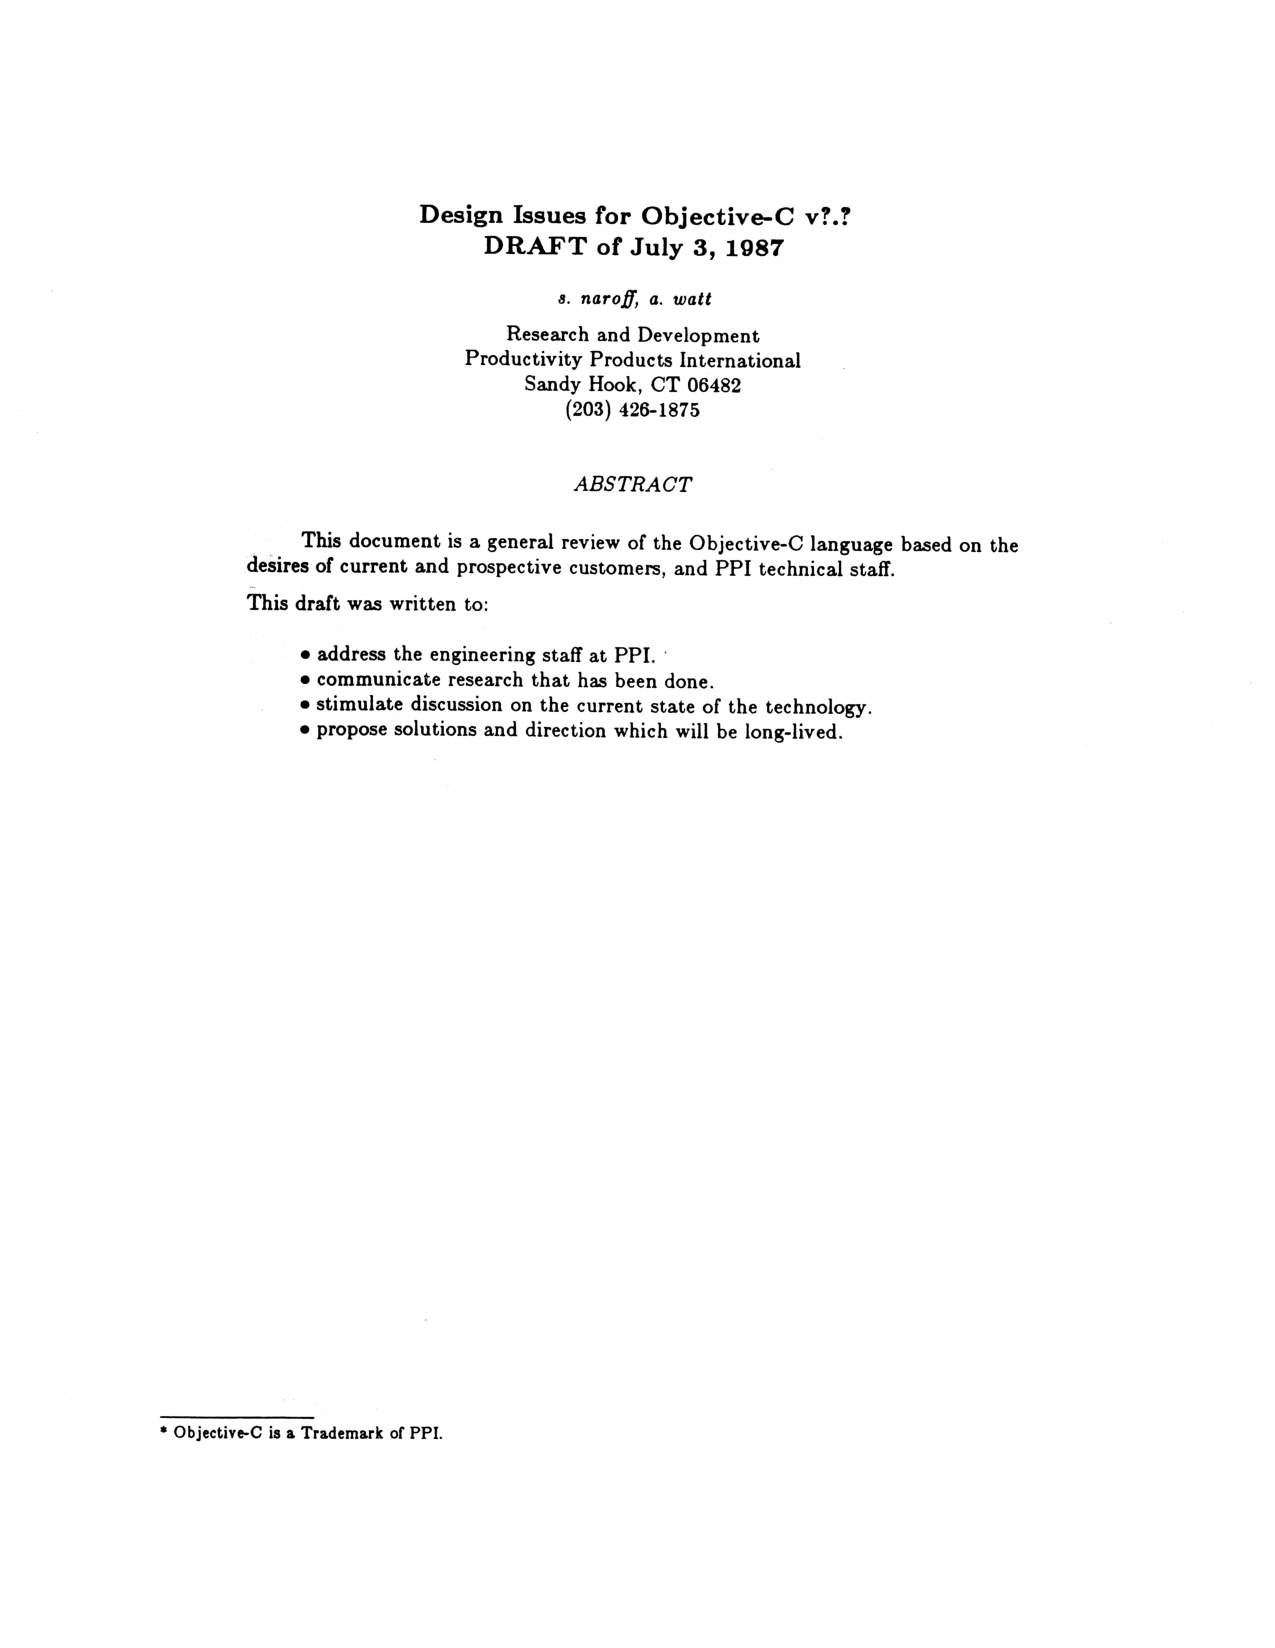
\includepdf[pages=1, 
width=\linewidth,
link=true,
pagecommand={\section{Historical document: Design Issues for Objective-C DRAFT of July 3, 1987, S. Naroff, A. Watt, PPI}
\label{appendix_NaroffWatt1987}}
]
{SNaroffAWatt1987ObjCDesignIssues.pdf}
\includepdf[pages={2-}, 
width=\linewidth, 
link=true,
pagecommand={}]
{SNaroffAWatt1987ObjCDesignIssues.pdf}

\includepdf[pages=1, 
landscape=false,
angle=90,
width=\linewidth, 
link=true,
pagecommand={\section{Historical document: Objective-C v.4.0 charts, Stepstone, 1988}
\label{appendix_StepstoneObjC4Charts}}
]
{Stepstone1988ObjC4_0Charts.pdf}
\includepdf[pages={2-last}, 
landscape=false,
angle=90,
width=\linewidth, 
link=true,
pagecommand={},
]
{Stepstone1988ObjC4_0Charts.pdf}

\includepdf[pages=1, 
width=\linewidth,
link=true,
pagecommand={\section{Historical document: Functional Specification: Class Declaration Syntax and Run-Time Selector Mapping in the Objective-C Language (spec.language), S. Naroff, c.1987}
\label{appendix_spec.language}}
]
{SNaroffSpec_language.pdf}
\includepdf[pages={2-last}, 
width=\linewidth,
link=true,
pagecommand={}]
{SNaroffSpec_language.pdf}

\includepdf[pages=1, 
width=\linewidth, 
link=true,
pagecommand={\section{Historical document: Design Notebook: Selector Mapping in the Objective-C Run-Time Support System (spec.runtime), S. Naroff, c.1987}
\label{appendix_spec.runtime}}
]
{SNaroffSpec_runtime.pdf}
\includepdf[pages={2-last}, 
width=\linewidth,
link=true,
pagecommand={}]
{SNaroffSpec_runtime.pdf}

%% Bibliography
\bibliography{HOPL-IV_ObjC}
\clearpage
\bibliographyNA{Nonarchival}

\end{document}
